%----------
%	CONFIGURACIÓN DEL DOCUMENTO
%----------

\documentclass[12pt,a4paper]{report} 
\let\iiint\relax

% MÁRGENES
\usepackage[
a4paper,
vmargin=2.5cm,
hmargin=3cm
]{geometry}

% INTERLINEADO
\renewcommand{\baselinestretch}{1.15}
\parskip=6pt

% COLORES
\usepackage[table]{xcolor}
\definecolor{azulUC3M}{RGB}{0,0,102}
\definecolor{gray97}{gray}{.97}
\definecolor{gray75}{gray}{.75}
\definecolor{gray45}{gray}{.45}

% CODIFICACIÓN Y FUENTES
\usepackage[utf8]{inputenc}
\usepackage[T1]{fontenc}
\usepackage{txfonts} 
\usepackage{microtype}

% IDIOMA (Inglés)
\usepackage[english]{babel} % Configurado a inglés
\usepackage[babel, english=american]{csquotes}
\AtBeginEnvironment{quote}{\small}

% AMSTEXT CONFLICT
\let\iint\relax
\let\iiint\relax
\let\iiiint\relax
\let\idotsint\relax
% PAQUETES MATEMÁTICOS Y GRÁFICOS
\usepackage{amsmath,amssymb,amsfonts,amsthm}
\usepackage{graphicx}
\usepackage{booktabs}
\usepackage{float}
\usepackage{array}
\usepackage{longtable}
\usepackage{tabularx}
\usepackage{multirow} 

\usepackage{caption}
\usepackage[capbesideposition=inside,subfloat]{floatrow}

% ENLACES (Cargar al final del preámbulo generalmente)
\usepackage{hyperref}
\hypersetup{colorlinks=true,
	linkcolor=black,
	urlcolor=blue}

% GENERACIÓN PDF/A
\usepackage[a-1b]{pdfx}

% DISEÑO DE PIE DE PÁGINA
\usepackage{fancyhdr}
\pagestyle{fancy}
\fancyhf{}
\renewcommand{\headrulewidth}{0pt}
\rfoot{\thepage}
\fancypagestyle{plain}{\pagestyle{fancy}}

% DISEÑO DE TÍTULOS (Capítulos y secciones)
\usepackage{titlesec}
\usepackage{titletoc}

\titleformat{\chapter}[block]
{\large\bfseries\filcenter}
{\thechapter.}
{5pt}
{\MakeUppercase}
{}
\titlespacing{\chapter}{0pt}{0pt}{*3}

% CHAPTER
\titlecontents{chapter}
[0pt]                               % Left indent
{\addvspace{1pc}\bfseries}          % Above code (spacing and bold)
{\thecontentslabel.\enspace\MakeUppercase} % Numbered entry format
{\MakeUppercase}                    % Numberless entry format (e.g. ACKNOWLEDGMENTS)
{\titlerule*[.7pc]{.}\contentspage} % Filler and page number

% SECTION
\titlecontents{section}
[1.5em]
{}
{\contentslabel{2em}}
{}
{\titlerule*[.7pc]{.}\contentspage}

% SUBSECTION
\titlecontents{subsection}
[3.8em]
{}
{\contentslabel{3em}}
{}
{\titlerule*[.7pc]{.}\contentspage}

% SUBSUBSECTION
\titlecontents{subsubsection}
[7em]
{}
{\contentslabel{4em}}
{}
{\titlerule*[.7pc]{.}\contentspage}


% DISEÑO DE TABLAS (Inglés)
\newcolumntype{P}[1]{>{\centering\arraybackslash}p{#1}}
\DeclareCaptionFormat{upper}{#1#2\uppercase{#3}\par}

\captionsetup*[table]{
	format=upper,
	name=TABLE, % Cambiado a TABLE
	justification=centering,
	labelsep=period,
	width=.75\linewidth,
	labelfont=small,
	font=small
}

% DISEÑO DE FIGURAS
\graphicspath{{imagenes/}} 

\captionsetup[figure]{
	format=hang,
	name=Fig.,
	singlelinecheck=off,
	labelsep=period,
	labelfont=small,
	font=small		
}

% NOTAS A PIE DE PÁGINA
\usepackage{chngcntr} 
\counterwithout{footnote}{chapter}

% LISTADOS DE CÓDIGO
\usepackage{listings}

\lstdefinestyle{estilo}{ frame=Ltb,
	framerule=0pt,
	aboveskip=0.5cm,
	framextopmargin=3pt,
	framexbottommargin=3pt,
	framexleftmargin=0.4cm,
	framesep=0pt,
	rulesep=.4pt,
	backgroundcolor=\color{gray97},
	rulesepcolor=\color{black},
	basicstyle=\ttfamily\footnotesize,
	keywordstyle=\bfseries,
	stringstyle=\ttfamily,
	showstringspaces = false,
	commentstyle=\color{gray45},
	numbers=left,
	numbersep=15pt,
	numberstyle=\tiny,
	numberfirstline = false,
	breaklines=true,
	xleftmargin=\parindent
}

\captionsetup*[lstlisting]{font=small, labelsep=period}
\lstset{style=estilo}
\renewcommand{\lstlistingname}{\uppercase{Code}} % Cambiado a CODE

% BIBLIOGRAFÍA (IEEE English)
\usepackage[backend=biber, style=ieee, isbn=false, sortcites, maxbibnames=6, minbibnames=1]{biblatex}
\addbibresource{sample.bib} 

% Configuración del índice 
\setcounter{tocdepth}{3}  % hasta subsubsección
\setcounter{secnumdepth}{3}

%-------------
%	DOCUMENTO
%-------------

\begin{document}
\pagenumbering{roman} 
	
%----------
%	PORTADA
%----------	
\begin{titlepage}
	\begin{sffamily}
	\color{azulUC3M}
	\begin{center}
		\begin{figure}[H] 
			% Asegúrate de que el logo existe en tu proyecto o comenta esta línea
			\makebox[\textwidth][c]{
\includegraphics[width=16cm]{logo_UC3M.png}}
		\end{figure}
		\vspace{2.5cm}
		\begin{Large}
			Degree in Data Science and Engineering\\
            Double Degree in Telecommunications Engineering and Data Science and Engineering\\
			 2025-2026\\ 
			\vspace{2cm}		
			\textsl{Data Science Project Final Report}
			\bigskip
			
		\end{Large}
		 	{\Huge Financial Transaction Fraud Detection: Securing the Industry with Artificial Intelligence}\\
		 	\vspace*{0.5cm}
	 		\rule{10.5cm}{0.1mm}\\
			\vspace*{0.5cm}
		\begin{Large}
			Silvia Díez\\
			Andrea López \\
            César Ramírez \\
            Enica King \\ 
            Emma Hernández 
            \\
		\end{Large}
	\end{center}
	\vfill
	\color{black}
	% LICENCIA CREATIVE COMMONS
    % Asegúrate de que la imagen existe o comenta la línea
	
\includegraphics[width=4.2cm]{creativecommons.png}\\ 
    This work is licensed under Creative Commons \textbf{Attribution - Non Commercial - Non Derivatives}
	\end{sffamily}
\end{titlepage}

% Aquí empezaría tu índice y contenido
\clearpage
\tableofcontents
\newpage


\pagenumbering{arabic}
\setcounter{page}{1}
\chapter{INTRODUCTION}
\section{Summary}
This project is a collaboration between the IBM company Bluetab and  students of the Charles III of Madrid University for the Data Science Project class. Providing students with professional mentorship allowed for application of theoretical concepts to a project in a professional context. Over the course of four months, these main four tasks were carried out: data pre-processing, development of a technical solution, analysis of legal and ethical aspects and analysis of the economic feasibility of the proposed solution.

\section{Objectives}
The main goals of the project were to use advanced Machine Learning (ML) techniques in order to accurately classify cases of financial fraud. Doing so would improve the detection capacity of illegal activity, minimize economic losses, and strengthen banking and insurance by securing financial operations.

\section{Initial Obstacles}
In the first phases of the project, making the connection between the task at hand and the datasets provided by the Bluetab team was the biggest hurdle to overcome. The datasets contained uninterpretable variables, misleading columns, and class imbalances that required a great effort in the preprocessing stage. Furthermore, establishing our working methods and workflow was also difficult since this project needed more documentation and organization than any previous project, and our groupmates and topic were assigned rather than freely chosen.

\section{Timeline}
Key events of the project are mapped out below; meetings with the company and with team members have not been listed.
\begin{figure}[H]
    \centering
    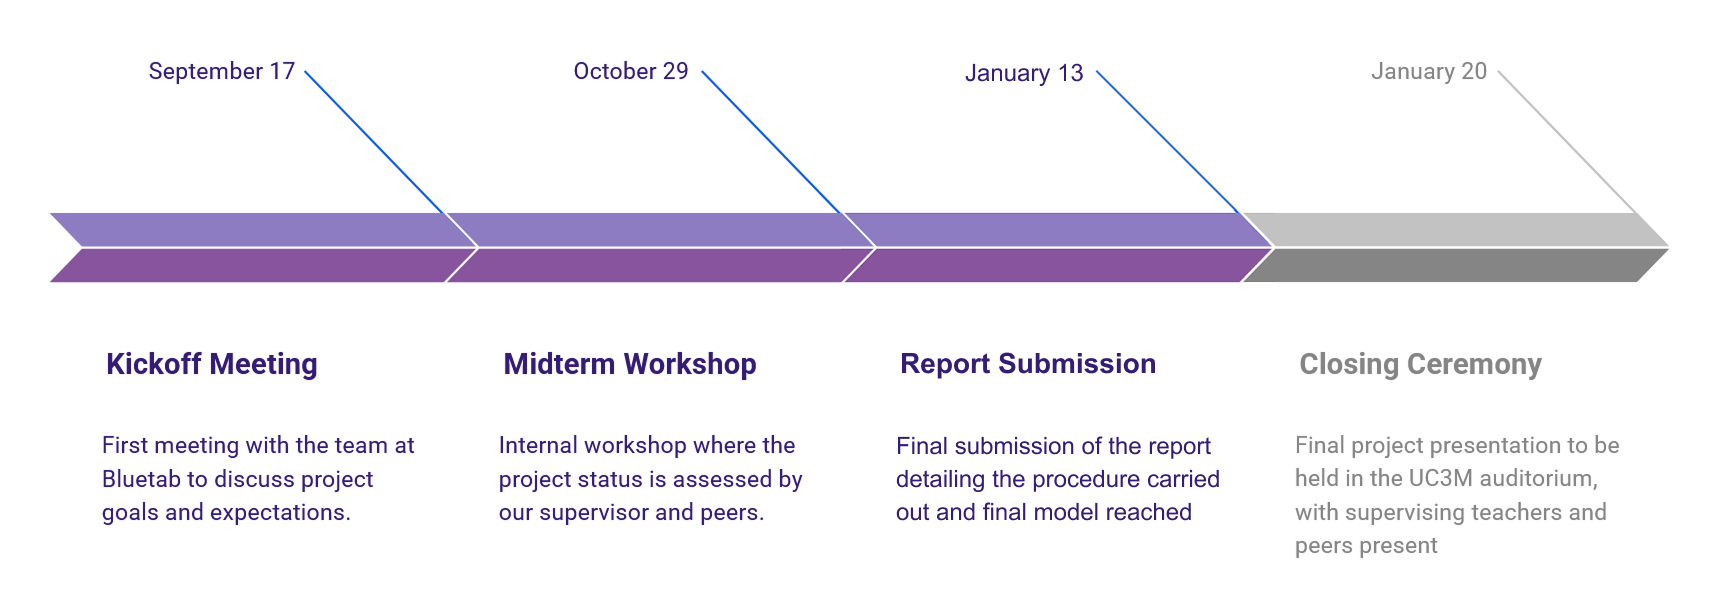
\includegraphics[width=1\textwidth]{Timeline Final.png}
    \caption{Project timeline.}
    \label{fig:timeline}
\end{figure}
\section{Background}
Nowadays, the modern financial system, including traditional and digital banks, as well as the insurance sector, operates in an environment of high complexity, which is regulated and characterized by a growing number of digital transactions.
The number of digital transactions has grown exponentially over the past few years, due to the facilities offered to customers worldwide dealing with e-commerce, and the popularization of contactless payment. But not everything is as good as it seems, as it has happened all over in the history of mankind; some people are willing to take advantage of those who are more vulnerable, who do not know someone who has not been targeted for a fraudulent action, such as identity theft, cloning the credit card, simulated transactions, money laundering or simply being catfished.

This represents a serious issue for financial entities, as they are currently operating on millions of daily transactions, for which just a small fraction of those could imply significant losses. That is why even though these transactions only represent 0.1 percent of the total volume, they can cost companies millions of dollars. This is the main reason why early and accurate detection is such an important and top-priority strategy.
\subsection{Most common fraud types}
For this project, instead of directly tackling the given data, we decided to first understand the topic we were going to deal with for the next couple of months, so we did some research on the most common types of fraud in the financial sector:
\begin{itemize}
    \item Credit Fraud: unauthorized access or cloning of credit/debit cards. 
    \item Identity Fraud: opening accounts or requesting credit access by means of false personal data.
    \item Internal Fraud: done by employees or partners.
    \item Money Laundering: complex movements to occult the illicit origin of the money. 
    \item Transaction Fraud: the one we are most interested in; account manipulation, or being tricked, such as phishing.
\end{itemize}

As each type has its own different patterns, the Machine Learning models must be able to detect anomalies for every context, such as the amount, the location, the schedule, or the client.
\subsection{Regulation and obligations}
We did not want to focus only on the basics, as we are expected to return not only a suitable model that is able to detect fraudulent transactions, but we are also committed to developing a design on Risk Management and Prevention Strategies based on what we have obtained during the project. That is why we have also done some research on how the financial sector is regulated and what legal obligations they must comply with. And what we have discovered is something we could think of, knowing that millions of dollars are at risk on a daily basis, it is a strong and well-regulated environment, in which the institutions must comply with international laws, such as :
\begin{itemize}
    \item KYC (Know Your Customer): Identification and verification of customers
    \item AML (Anti-Money Laundering): money laundering prevention
    \item Open Banking (only in Europe): API security and reinforced authentication
\end{itemize}
This implies that the fraud detection systems must not only be precise, but also be explainable and auditable. The transparency of the ML models is a technical and normative must-have.

\subsection{Technological Environment}
We also studied what the state-of-the-art was for financial institutions in recent years:
\begin{itemize}
    \item Real-time analysis systems based on Big Data
    \item Combined use of ML models and Deep Learning for detecting anomalies 
    \item Hybrid architectures (on-premise + cloud) for security and scalability
    \item Incorporating analytic dashboards for executive monitoring 
\end{itemize}

For the project team, being familiar with this new environment implied understanding that technical decisions are conditioned by laws and regulations, cybersecurity, and the criticality of financial operations.

\chapter{EXPLORATORY DATA ANALYSIS}
After the midterm workshop on October 29 we were given new datasets from Bluetab. Up until then we had already performed an exploratory analysis and started feature selection on the initial datasets, detailed in the midterm report. From this point on we will present our findings from these six new raw datasets.

\section{Raw Data Exploration}

\subsection{Overview of the raw sources}
We were given \textbf{six raw datasets}, each providing different information regarding bank transactions. 
\begin{itemize}

    \item \textbf{transactions\_dirty.csv} – A \textbf{286,315 $\times$ 33} dataset which contains anonymized information 
    about individual transactions including three unique identifiers:

    \begin{center}
    \begin{tabular}{|l|l|p{8cm}|}
        \hline
        \textbf{Variable} & \textbf{Type} & \textbf{Description} \\
        \hline
        \textit{V1 -- V28} & Numeric (continuous) & Anonymized features resulting from a PCA transformation of original data. \\
        \hline
        \textit{transaction\_id} & String & ID of the observed transaction. \\
        \hline
        \textit{customer\_id} & String & ID of the bank customer linked to the transaction. \\
        \hline
        \textit{device\_id} & String & ID of the device used to perform the transaction. \\
        \hline
    \end{tabular}
    \end{center}

    \item \textbf{locations\_dirty.csv} – A \textbf{286,315 $\times$ 6} dataset which includes geographical and merchant variables 
    for each transaction in addition to the transaction identifier:

    \begin{center}
    \begin{tabular}{|l|l|p{8cm}|}
        \hline
        \textbf{Variable} & \textbf{Type} & \textbf{Description} \\
        \hline
        \textit{ip\_address} & String & IP address associated with the transaction. \\
        \hline
        \textit{country} & Categorical & Country where the transaction occurred. \\
        \hline
        \textit{city} & Categorical & City where the transaction occurred. \\
        \hline
        \textit{zip\_code} & Categorical & Postal code of the transaction location. \\
        \hline
        \textit{merchant} & Categorical & Merchant's name. \\
        \hline
    \end{tabular}
    \end{center}

    \item \textbf{customers\_dirty.csv} – A \textbf{1,000 $\times$ 8} dataset which contains customer information 
    within the following variables, including the customer identifier:

    \begin{center}
    \begin{tabular}{|l|l|p{8cm}|}
        \hline
        \textbf{Variable} & \textbf{Type} & \textbf{Description} \\
        \hline
        \textit{name} & String & Customer's name. \\
        \hline
        \textit{age} & Numeric & Customer's age. \\
        \hline
        \textit{email} & String & Customer's email address. \\
        \hline
        \textit{phone} & String & Customer's phone number. \\
        \hline
        \textit{country} & Categorical & Customer's country of residence. \\
        \hline
        \textit{credit\_score} & Numeric & Customer's creditworthiness score. \\
        \hline
        \textit{join\_date} & Date & Date when the customer opened the account. \\
        \hline
    \end{tabular}
    \end{center}

    \item \textbf{flags.csv} – A \textbf{286,315 $\times$ 4} dataset which contains  information 
    about transactions that could be flags for it being fraudulent:

    \begin{center}
    \begin{tabular}{|l|l|p{8cm}|}
        \hline
        \textbf{Variable} & \textbf{Type} & \textbf{Description} \\
        \hline
        \textit{transaction\_id} & String & ID of the observed transaction. \\
        \hline
        \textit{is\_foreign\_tx} & Binary (0/1) & 0 indicates the transaction comes from the same country while 1 indicates the transaction is foreign. \\
        \hline
        \textit{in\_night\_tx} & Binary (0/1) & 0 indicates the transaction was performed during the day while 1 indicates at night. \\
        \hline
        \textit{is\_high\_amount} & Binary (0/1) & 0 indicates a low amount transaction while 1 indicates a high amount transaction. \\
        \hline
    \end{tabular}
    \end{center}

    \item \textbf{time\_table.csv} – A \textbf{286,315 $\times$ 7} dataset which contains time related information 
    about transactions with the following variables:

    \begin{center}
    \begin{tabular}{|l|l|p{8cm}|}
        \hline
        \textbf{Variable} & \textbf{Type} & \textbf{Description} \\
        \hline
        \textit{transaction\_id} & String & ID of the observed transaction. \\
        \hline
        \textit{timestamp} & String & Time stamp of the transaction. \\
        \hline
        \textit{hour} & Numeric & Hour of the day the transaction took place in. \\
        \hline
        \textit{day\_of\_week} & Categorical & Day of the week the transaction took place in. \\
        \hline
        \textit{is\_weekend} & Binary (0/1) & 0 indicates the transaction took place during the week while 1 indicates it took place over the weekend. \\
        \hline
        \textit{month} & Binary (0/1) & Month the transaction took place in. \\
        \hline
        \textit{time\_of\_day} & Categorical & Time of the day the transaction took place at (e.g., Night, Morning). \\
        \hline
    \end{tabular}
    \end{center}

    \item \textbf{devices.csv} – A \textbf{100 $\times$ 5} dataset which contains information about devices used to perform the transactions with the following variables:

    \begin{center}
    \begin{tabular}{|l|l|p{8cm}|}
        \hline
        \textbf{Variable} & \textbf{Type} & \textbf{Description} \\
        \hline
        \textit{device\_id} & String & ID of the device used to perform the transaction. \\
        \hline
        \textit{device\_type} & Categorical & Type of device (e.g., Desktop, ATM). \\
        \hline
        \textit{os} & Categorical & Operation system of device (e.g., macOS, Android). \\
        \hline
        \textit{browser} & Categorical & Browser of device (e.g., Chrome, Firefox) \\
        \hline
        \textit{is\_mobile} & Binary (0/1) & 0 indicates the transaction is not performed from a mobile phone while 1 indicates it is. \\
        \hline
    \end{tabular}
    \end{center}
\end{itemize}
    
\subsection{Variable grouping}
Having these six initially separated datasets provided a \textbf{clearer and more structured understanding} of the data landscape we were dealing with. This allowed us to understand the \textbf{role and relevance} of each variable and group them into different categories.
\begin{itemize}
    \item \textbf{Transactional} \\
    Formed by \textit{time}, \textit{amount}, and the 28 anonymized components (\(V1\)--\(V28\)).

    \item \textbf{Identifiers and keys} \\
    In this group we find the \textit{transaction\_id}, \textit{customer\_id}, and \textit{device\_id}. 
    These variables will be crucial for later dataset aggregation and leakage control in model evaluation.

    \item \textbf{Geolocation and merchant attributes} \\
    This group includes categorical fields with moderate to high numbers of categories such as 
    \textit{ip\_address}, \textit{country}, \textit{city}, \textit{zip\_code}, \textit{is\_foreign\_tx} and \textit{merchant}. 
    They help describe the merchant context of each transaction and keep track of the “normal” behavior of customer transactions.

    \item \textbf{Temporal Features} \\
    This group is derived from the raw \textit{timestamp} and captures the "when" of the transaction with variables such as
    \textit{hour}, \textit{day\_of\_week}, \textit{month}, \textit{time\_of\_day}, \textit{is\_weekend} and \textit{is\_night\_tx}. 
    They are vital for capturing trends and off-hour fraud attempts.

    \item \textbf{Customer and Device attributes} \\
    Formed by variables such as \textit{age}, \textit{country}, and \textit{credit\_score} which help group customers due to their risk potential, 
    \textit{join\_date} that provides recency information, contact fields like \textit{email} and \textit{phone} which can flag data-entry patterns, and technical environment features such as \textit{device\_type}, \textit{os}, \textit{browser}, and \textit{is\_mobile}.
\end{itemize}

\section{Data Merge}
After analyzing each dataset, we decided to merge them in order to work with them. Before merging, we identified and solved inconsistencies that could compromise data integrity. In particular, we detected duplicated transaction\_id, which we carefully reviewed and cleaned removing those whose client\_id did not exist in customers\_df. This avoided null joins and ensured correct data merging. 
After merging, we standardized column names and adjusted variable data types (for instance, ensuring that numerical variables were in the correct format and categorical ones were properly encoded).
As a result we obtained a dataset of 286315 rows and 58 features.

\subsection{Class imbalance}
From this complete dataset we observe \textbf{284,068 non-fraudulent} entries (\textit{Class} = 0) and \textbf{2,000 fraudulent} entries (\textit{Class} = 1), resulting in a fraud rate of 0.7\%. Therefore, we concluded that our target variable \textit{Class} was severely imbalanced.
This is a recurrent problem in fraud detection which we will solve in the following stages of our exploration in order to accomplish accurate and realistic classification results. One of the main solutions we contemplated was the creation of synthetic data entries from existing data.

\subsection{Univariate and bivariate characteristics}
To better understand the \textbf{statistical behaviour} of individual variables and the relationship between them we performed both univariate and bivariate examinations. The univariate analysis helped us study the \textbf{distribution} of each feature, which allowed us to identify skewed variables, potential outliers, and the need for normalization or transformation. On the other hand, the bivariate analysis focused on \textbf{relationships} between each variable and the target, which could help us recognize potential patterns and dependencies.

After performing univariate analysis for all \textbf{numerical features} we drew the following conclusions. The \textit{amount} is highly right-skewed meaning most of the transactions are of low quantity with a long tail extending to high quantity representing rare high-value transactions. This is further supported by the distribution of the engineered flag \textit{is\_high\_amount}. 
The \textit{age} shows a relatively uniform distribution, which indicates a balanced representation of all age groups. The \textit{credit\_score} displays a bell-shaped distribution with values concentrated between 500 and 850 points, which represents a realistic distribution. The PCA-like variables \(V1\)--\(V28\) show approximately symmetric and centered distributions around zero, some being more dispersed than others, yet in accordance with standardized transformations having mean and variance around 0 and 1 respectively.
Finally, the temporal features, \textit{hour} shows specific peak periods of activity, moreover, we observe that \texit{is\_night\_tx} and \texit{is\_weekend} provide critical context for transaction timing.
\begin{figure}[H]
    \centering
    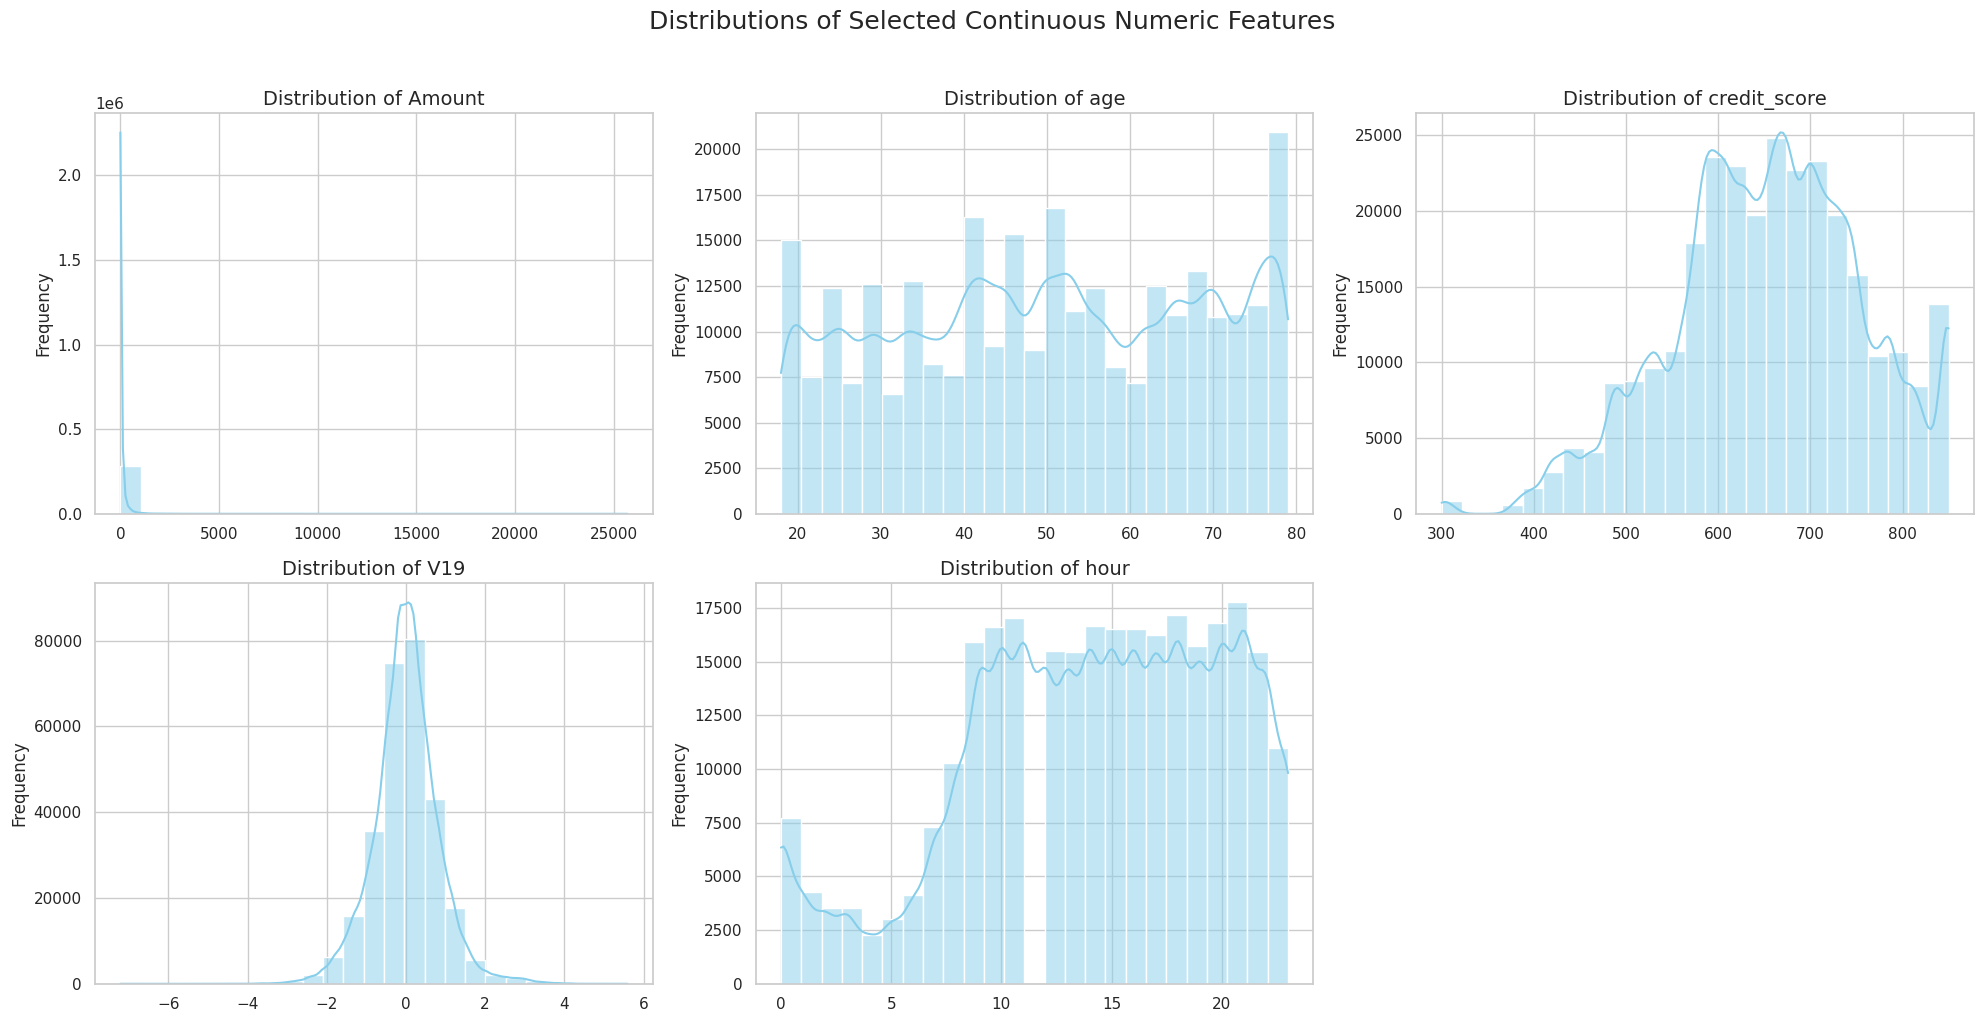
\includegraphics[width=1\textwidth]{univariate_numeric.png}
    \caption{Distribution of numeric features.}
    \label{fig:univariate_numeric}
\end{figure}
For the categorical features we highlight the following. The customer’s \textit{country} shows a highly long-tailed distribution including a large number of countries with very different frequencies, a small group dominating the dataset and the rest of countries appearing with progressively smaller counts. Unlike the latter, the merchant’s \textit{country} distribution shows a small number of countries with equal frequencies across the dataset, appearing to be balanced and uniform. Similarly, \textit{city} displays a semi-uniform distribution, counts being relatively even. The distribution of \textit{zip\_code} is relatively uniform, suggesting most zip codes occur at similar frequencies. Finally, technical metadata variables such as \textit{os} and \textit{browser} show clear majorities, which will be essential for identifying anomalies.
\begin{figure}[H]
    \centering
    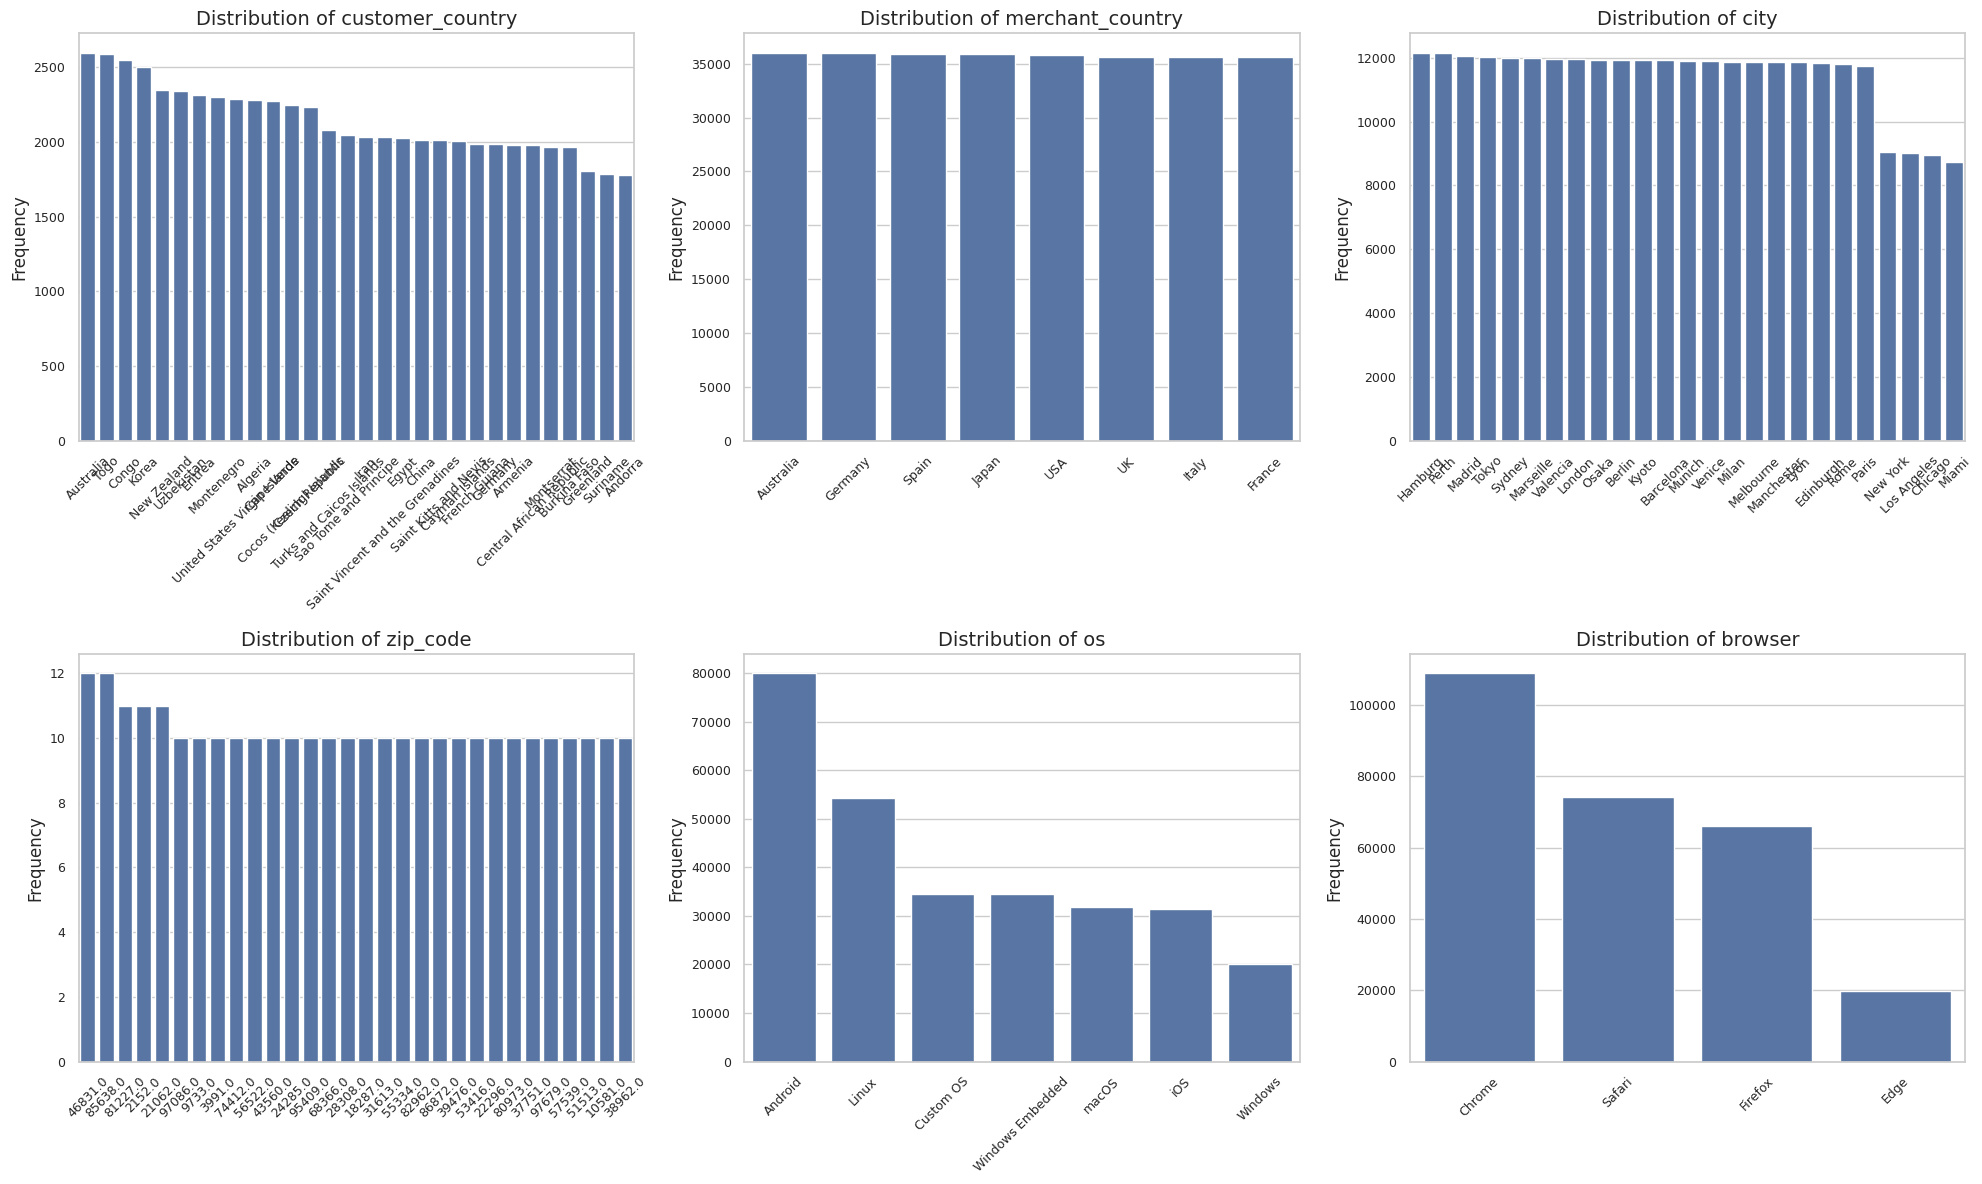
\includegraphics[width=1\textwidth]{univariate_categorical.png}
    \caption{Distribution of categorical features}
    \label{fig:univariate_categorical}
\end{figure}

To study the bivariate relationships we plotted the variables against the target \textit{Class}. The plots convey that fraudulent transactions tend to appear more around lower monetary values. For the rest of the variables, only minimum differences between classes are shown. As we have covered before, we are facing a high class imbalance problem. Therefore, while the classes may appear to behave similarly across demographic or geographic features, we will need to make use of advanced modeling and sampling techniques to uncover the subtle deviations that characterize fraudulent transactions.

\subsection{Missing values}
The next step was to perform a missing value analysis. This revealed several null values across different categories, primarily coming from the data merging process where transaction records were joined with customer profile tables. In Figure 2.1 we can observe the columns and rows with missing values. 
\begin{figure}[H]
    \centering    
\includegraphics[width=0.8\textwidth]{missing_values.png}
    \caption{Location of missing values for each feature.}
    \label{fig:missing_values}
\end{figure}

To handle this, we took the following actions:
\begin{itemize}
    \item \textbf{Removal of Incomplete Customer Profiles:} We identified a specific subset of 247 records where customer information (such as \textit{name}, age, \textit{customer\_country}, \textit{credit\_score}, and \textit{join\_date}) were entirely missing. After performing some analysis, we confirmed that these records did not contain any fraudulent instances (\textit{Class} == 0). Consequently, these rows were removed.

    \item \textbf{Imputation of Categorical Features:} Several variables showed partial missingness, specifically \textit{zip\_code}, \textit{browser}, \textit{email}, and \textit{phone} (with null rates ranging from 2\% to 10\%). To preserve these transactions while maintaining data integrity, we imputed missing values with the placeholder "Unknown". This way, we ensured the cases remain distinguishable for the model, as the absence of this information could be a predictive feature in fraud detection.
\end{itemize}

\subsection{Outliers}
Next, we conducted an outlier analysis to identify anomalous values that could distort the statistical properties of the dataset or bias predictive modeling. We used the Interquartile Range (IQR) to quantify the number and percentage of outliers for each numerical feature.

This revealed a significant number of observations in the \textit{V1-V28} and \textit{Amount} variables lying far outside the IQR. However, given the financial context, we opted to keep these unusually high values since they could be related to fraudulent behavior. 

In addition, negative values were checked across all numerical variables, and none were considered invalid based on the context of the data. The variable age was validated to ensure all entries fell within realistic bounds (18 to 79 years old).

Finally, categorical and binary variables were examined to confirm that all encoded categories and binary indicators (0/1) aligned with their expected domains, ensuring overall data quality and consistency before correlation and feature analysis.

\subsection{Correlations}
For the correlation analysis, we attempted to understand the linear relationships between our variables and the likelihood of fraud. We computed a correlation matrix focusing on the \textit{Class} target. 

From the results, we observed that while most variables show weak linear correlations certain \textit{V1-V28} variables exhibited significant positive and negative relationships with fraudulent activity. Specifically, \textit{V11}, \textit{V4}, and \textit{V2} had the strongest positive correlations with \textit{Class}, meaning as these values increase, the probability of fraud tends to rise. Conversely, \textit{V17}, \textit{V14}, and \textit{V12} exhibited strong negative correlations, which can serve as important indicators for non-fraudulent transactions when their values are high.

The correlation heatmap also showed that the anonymized features \textit{V1–V28} had very low pairwise correlations, which led us to think they were principal components. In addition, the contextual variables \textit{Amount}, \textit{age}, and \textit{credit\_score} also displayed low correlation with the V-features, suggesting they provide complementary insights about each transaction. On the other hand, the interaction of features like \textit{hour} and \textit{is\_night\_tx} with the possible PCA components suggested that fraud occurs in specific "pockets" of the feature space.

Finally, since no strong correlations were observed, we do not have multicollinearity problems, which is beneficial for model training.

\chapter{FEATURE ENGINEERING}

\section{Feature Creation}
In this phase, we transformed the raw data into more predictive signals, specifically focusing on capturing the behavioral context of a transaction rather than just its individual values. We have categorized these into five  main subsections.\\

\textbf{Temporal and Cyclical feature engineering}\\
Since our dataset spans only two days, we focus on short-term temporal patterns rather than weekly or monthly seasonality. This means we engineered features that capture hourly behavior, time-of-day, night activity, and account tenure. All of which can help detect abnormal transaction timing.

Therefore, we created the variable \textit{days\_in\_bank} to know how many days a user has been in the bank, encoded \textit{hour} as cyclical variables (sin/cos), and created flags for night, morning, afternoon, and evening.\\

\textbf{Transaction dynamics}\\
We engineered features to describe how quickly and frequently customers interact with the system.

By sorting records by customer and time, we calculated the time elapsed since the last transaction \textit{secs\_since\_prev\_tx} since high-velocity bursts of transactions are often linked to automated fraud.

Additionally, we calculated  \textit{tx\_per\_customer} and \textit{tx\_rate} to differentiate between high-activity power users and anomalous spikes in behavior.\\

\textbf{Merchant and Country risk}\\
This section focuses on features that capture geographical and merchant-level fraud patterns.
Fraudulent transactions often cluster around specific merchants or countries with higher risk levels. By quantifying these risks, we allow the model to learn where fraud is more likely to occur.

We created \textit{merchant\_fraud\_rate}, the average fraud rate per merchant based on historical data; \textit{country\_fraud\_rate}, the average fraud rate per merchant country; \textit{geo\_anomaly}, the flag equal to 1 when the merchant and the customer are from different countries.\\

\textbf{Device and Technical Consistency}\\
These features capture anomalies in how customers interact with the system. Fraudsters often use different devices, browsers, or shared IP addresses compared to legitimate users. Sudden changes in device or browser may indicate account takeover and shared IPs often appear in coordinated fraud attacks

We created \textit{main\_device} and  \textit{main\_browser} which are the most frequently used device and browser by each customer, respectively, 
\textit{device\_change} and \textit{browser\_change} which flag if the current transaction uses a different device or browser, and finally 
\textit{shared\_ip} to flag equal to 1 when the same IP address is used by multiple customers.\\

\textbf{Transaction Amount Behavior}\\
These features describe how the transaction amount relates to typical spending patterns. Fraudulent transactions often involve unusually high amounts compared to normal activity.

We created \textit{amount\_log} which is the logarithmic transformation of the transaction amount, used to reduce skew and make extreme values less dominant, and \textit{is\_outlier\_amount} binary variable equal to 1 if the transaction amount is unusually high compared to the global distribution.\\

After this feature expansion we were left with 76 variables.

\section{Insights}
Following the feature engineering process, several critical insights were observed from the data's behavior.

With respect to the \textbf{temporal and cyclical patterns}, the 48-hour window shows a balanced distribution for \textit{is\_weekend} (\≈51\%), while the heterogeneous distribution of transaction hours suggests that cyclical encoding could be necessary to capture night-time activity dips.

When focusing in \textbf{customer tenure maturity}, the population is heavily skewed toward long-term clients, with approximately 68.5\% having a tenure of over two years. 

About \textbf{geographic and merchant} anomalies, the \textit{geo\_anomaly} flag showed extremely low variability (99.6\% cross-border), suggesting limited predictive value. Conversely, the high fraud rates found in specific merchants and countries indicate significant predictive potential but we need to make sure there is no data leakage.

With respect to the \textbf{technical consistency} we find high frequencies of \textit{device\_change} (70.9\%) and \textit{browser\_change} (61.9\%) were observed, which may signal session diversity or potential account takeovers. Although \textit{shared\_ip} is rare (0.01\%), it is identified as a potentially strong signal for coordinated fraud.

Finally, within transactional and behavioral dynamics, logarithmic normalization of amounts successfully managed the heavy-tailed distribution, while features like \textit{secs\_since\_prev\_tx} and \textit{tx\_rate} effectively capture high-intensity "burst" patterns typical of fraudulent activity.

\section{Studying Leakage}
Our study of leakage focused on features derived from target statistics, specifically those quantifying risk levels. We analyzed variables \textit{merchant\_fraud\_rate} and \textit{country\_fraud\_rate}, since they were initially calculated as the mean of the \textit{Class} variable for each merchant and country across the entire dataset. By examining the relationship between these rates and the target variable, we concluded that they introduced direct class leakage. To ensure the integrity of the predictive system, we decided to drop these variables entirely from the final feature set. 

\chapter{DATA EXPANSION}
\section{Four Initial Datasets}
Before we started the modeling process we decided to expand our dataset to obtain 500,000 observations in four different ways. We did this as an attempt to combat our high class-imbalance problem by generating new samples from the ones we already had. As a result we obtained the following four datasets which will be used in different models depending on their nature:

\begin{itemize}
    \item Random sample creation without taking into account the new observations class.
    \item Same imbalanced class proportion as before(99.3\% - 0.7\%)
    \item 66.6\% - 33.3\% Proportion
    \item 50\% - 50\% Proportion
\end{itemize}

\section{Eight Final Datasets}
After an initial take on modeling, using these four initial datasets, our results were not what we were aiming for. We came to the conclusion that some correlations between the PCA variables could be affecting this model behavior. Therefore, we studied these correlations and dropped the variables with relationships between them. After this, we created another four new datasets to use in our models with the expectation of a better result.

\chapter{MODELING}

\section{Methodology: Evolution of Validation Strategy}

\subsection{Initial Diagnostic: Overfitting problem}
At first, we trained models that gave suspicious results ($AUC = 1$). After studying what could be causing this inconsistency, we realised that the problem was the strategy of splitting the data in train and test set. The conventional random way of splitting the data did not respect the sequential nature of financial transactions.

\subsection{Solution: Temporal Split and Generation of Datasets}
To solve this problem, we implemented a validation temporal split, training with one day (past) and testing with the remaining day (future). We then created the 8 dataframes mentioned before, and started training.

\subsection{Evaluation strategy}
Since we have very imbalanced datasets, we decided not to use Accuracy as the principal metric. Instead, we prioritize metrics that are capable of detecting the minority class (fraud).

\begin{description}
    - F2-Score: Principal selected metric. This metric considers Recall and Sensitivity, giving more weight to Recall, so that it penalizes more the false negatives, rather than penalizing equally false negatives and false positives.
    \newline
    - AUC-PR (Area under the curve Precision-Recall): Very important for imbalance datasets.
    \newline
    - Recall and Precision: We analyze them individually to find the optimal threshold.
\end{description}

\section{Feature and Data Selection}

\subsection{Step 1: Selection of Best Dataframes}
We trained a Random Forest for each dataset using the 28 anonymized variables which we suspected came from a PCA, so that the model was not too complex. We chose these variables because were the ones that had more correlation with the class, and we were obtaining good enough results for the initial models.

After comparing the metrics for every dataset. The best results were obtained by the dataframe with the same proportion (\texttt{df\_exp\_same\_prop}) as the original one and the one with random proportion (\texttt{df\_exp\_random}). Since they had very similar metrics, we decided to keep both of them and compare them afterwards.

\subsection{Step 2: Feature selection}
In order to select more features in addition to the anonymized ones, we trained a LightGBM model to identify the most relevant features and avoid noise. This resulted in adding two new variables: the customer’s country (\texttt{customer\_country}), and the amount of the transaction in logarithmic form (\texttt{amount\_log}).

\section{Modeling and Final Results}
After selecting the final dataframes, we trained a Random Forest and a LightGBM model for both dataframes. In both of them, the dataset \texttt{df\_exp\_same\_prop} performed better. Thus, we decided to keep working with this dataset.

\subsection{Models}
We trained different ensemble models such as Random Forest, LightGBM, XGBoost and Catboost. We also trained a Logistic Regression model and compared the metrics. The best results were obtained with Random Forest.

\subsection{Hyperparameter Tuning}
In order to improve the Random Forest, we implemented a hyperparameter exhaustive search with Randomized Search Cross Validation. This resulted in a slightly worse F2-score and Recall, which could make sense due to overfitting. Thus, we kept the Random Forest model with predefined hyperparameters. The confusion matrix of the final model is the following: 
\begin{figure}[H] 
    \centering
    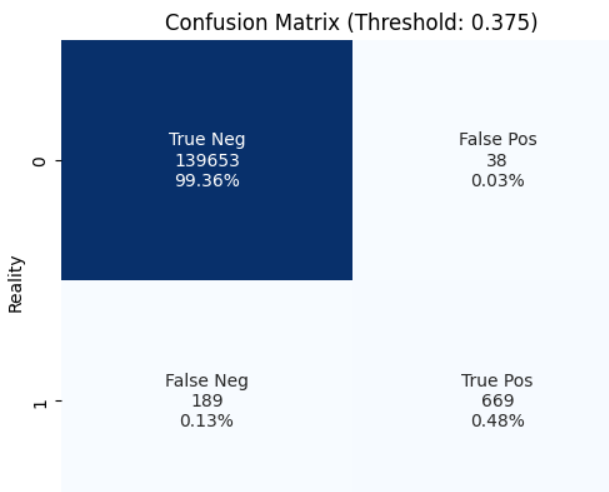
\includegraphics[width=0.8\textwidth]{imagenes/confusion_matrix.png} 
    
    \caption{Confusion Matrix of Final Model}
\end{figure}

\section{Conclusion}
The development of the fraud detection model demonstrated that the election of a robust validation strategy is as critical as the algorithm’s complexity. The identification of the overfitting problem led to a decisive change in the data division for testing.

The key giveaways from our experimental process include:

\begin{description}
    - Data Consistency: The dataframe used for training maintained the original proportions of the classes, and outperformed the manipulated distributions, suggesting that the model learns best from the natural frequency of fraud cases.
    \newline
    - Feature Relevance: Apart from the anonymized PCA variables, the feature selection assisted by LightGBM validated the importance of adding some new variables, enriching the predictive capability of the model.
    \newline
    - Model Selection: Random Forest demonstrated the best balance of precision and recall for this specific dataset.
    \newline
    - Metric Prioritization: By optimizing F2-Score, we successfully aligned the model's performance with the business need to minimize False Negatives (missed fraud cases), even at the cost of slightly lower precision.
\end{description}

Lastly, the study concludes that the Random Forest model with predefined hyperparameters serves as the optimal solution. The attempt to do a fine hyperparameter tuning led to a small degradation of the metrics, indicating that the base model offers a better capacity of generalization.


\chapter{DASHBOARD}

\section{Purpose and Role of the Dashboard}

Following development of the data pipeline and fraud detection models, a key challenge is to communicate results in a way that is useful for the different stakeholders. Machine learning outputs are not valuable unless they are translated into indicators, trends and visual explanations.  For this reason, one of the main goals of this project for Bluetab and our team, was to create an interactive web-based dashboard.

It acts as an interface between analytics and business decisions. Users can now monitor transactions, identify fraud patterns and assess model outputs without requiring the technical skills for direct interaction with the code or datasets.

The dashboard is designed for three different user profiles: 
\begin{itemize}
    \item\textbf{Business and executive users}, who need a high level view of fraud risk and volume.
    \item \textbf{Risk and compliance teams}, who need transparency and traceability.
    \item \textbf{Analysts and data scientists}, who need detailed exploration and performance metrics. 
\end{itemize}

Rather than a static report, the dashboard enables interactive exploration and keeps the analysis and prediction separate, providing a clear and quick understanding of our project.  However, we want to stress that this dashboard is a demo version, built for demonstration purposes.

\section{Design Principles}

The dashboard is structured as a multi-page application, where each page has a specific analytical purpose. The main design principles have been: 

\begin{itemize}
    \item \textbf{Clarity over complexity.} Each page focuses on a limited number of questions to avoid information overload.
    \item \textbf{Separation of observed data and predictions.} Avoid mixing ground-truth fraud labels with model predictions. 
    \item \textbf{Interactivity.} Filters and controls allow user to explore different data without changing the underlying models and datasets. 
\end{itemize}

\section{Dashboard Architecture}

The dashboard is divided into five main pages:
\begin{enumerate}
    \item \textbf{Overview}. High-level view of historical fraud data.
    \item \textbf{EDA}. Exploratory analysis comparing fraudulent and legitimate behavior.
    \item \textbf{Modeling and Performance}. Evaluation of the machine learning models and metrics.
    \item \textbf{Fraud Simulator}.Allows users to input transaction data and classify it using our best-performing model.
    \item \textbf{Strategies and Recommendations}. Business impact analysis, ROI evaluation, and fraud prevention recommendations.
\end{enumerate}

\section{Overview: Descriptive Monitoring of Fraud}
\begin{figure}
    \centering
    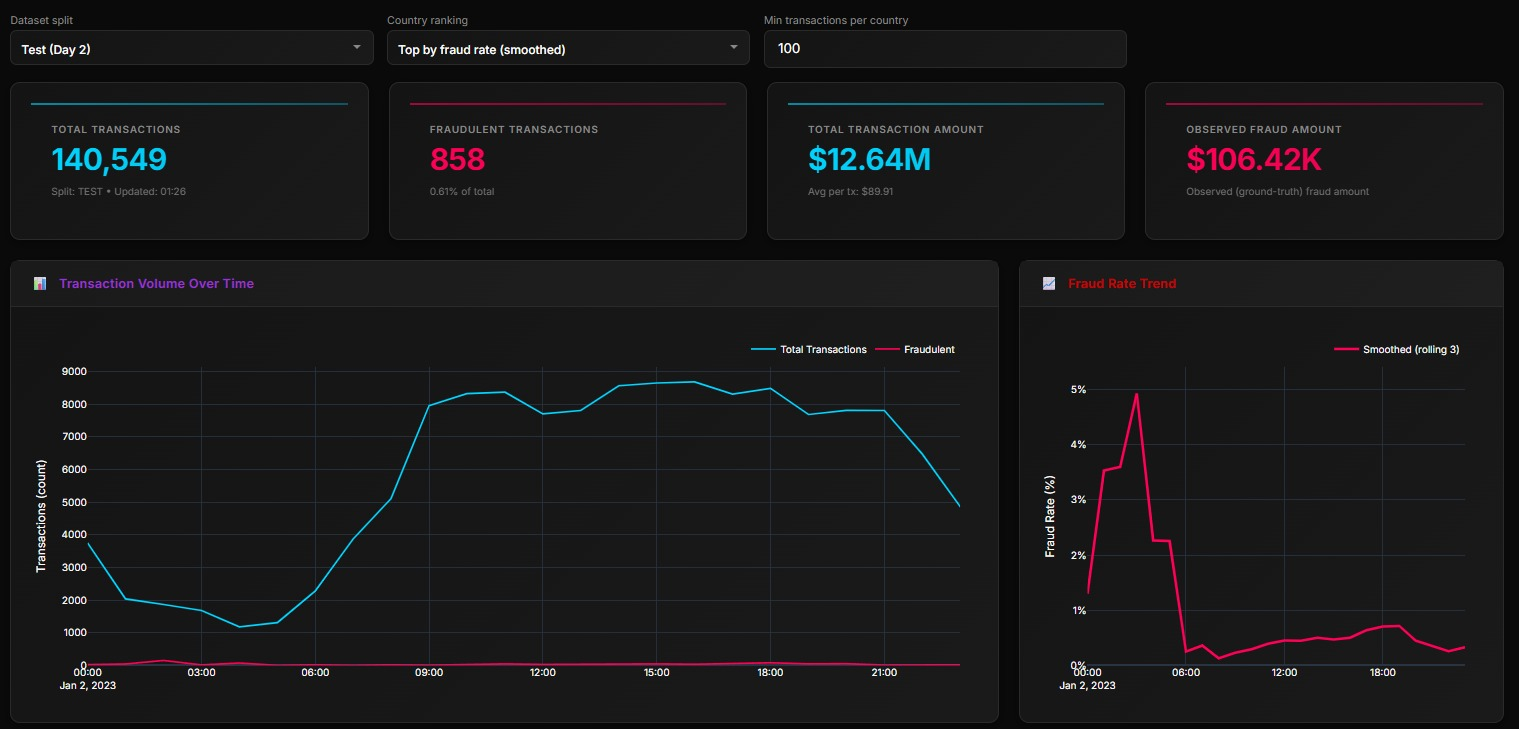
\includegraphics[width=1\linewidth]{imagenes/dashboard_overview.jpeg}
    
    
\end{figure}
\textit{Note: The dashboard pages are scrollable. For readability reasons, the screenshots shown do not capture the full vertical extent of each page.}

    \subsection{Objective of the Overview Page}

It is the entry point into our dashboard. Its main objective is to provide a fast and reliable snapshot of transaction activity and fraud patterns using historical ground-truth labels.

This page does not show any real-time predictions or model decisions. All metrics shown here are descriptive and based on already labeled data. This ensures that the user clearly understands the data and obtains context of the project before moving to classification analysis. It also allows for comparison between the training data, which has been synthetically generated during preprocessing, and the real test data (or a combination of the two).

The Overview answers three questions: 
\begin{itemize}
    \item How large is the transaction volume and fraud exposure?
    \item How does fraud evolve over time?
    \item Where is fraud geographically concentrated?
\end{itemize}

\subsection{Main Elements of the Overview Page}
    
\textbf{Key Performance Indicators (KPIs)}
At the top of the page, four KPI cards provide a concise summary of the selected dataset split:

\begin{itemize}
    \item Total Transactions
    \item Fraudulent Transactions
    \item Total Transactions Amount
    \item Observed Fraud Amount
\end{itemize}

The values are formatted for readability and updated dynamically based on user-selected filters.

\textbf{Temporal Analysis of Transactions and Fraud}
Two complementary time-based charts are included. The first shows transaction volume over time (two days) and compares total number of transactions with fraudulent ones. It is important to note that the training data has been expanded as explained previously.

The second graph displays the fraud rate trend using a rolling average. Smoothing is applied to reduce the short-term volatility and highlight meaningful changes in fraud behavior.

\textbf{Transaction Amount Distribution}
The distribution of transaction amounts is visualized using a histogram that separates legitimate and fraudulent transactions. To reduce skewness, a logarithmic scale is applied to the amount, as the transactions are concentrated at lower amounts, especially those that are corrupt.

\textbf{Geographical Risk Analysis}
Countries are ranked based on fraud risk using two alternative criteria: 
\begin{itemize}
    \item Fraud rate (smoothed). Percentage of transactions that are fraudulent in each country. Bayesian smoothing is applied to reduce noise from low-volume countries.
    \item Fraud amount (financial impact). Total monetary value of fraudulent transactions per country, representing the absolute financial exposure rather than the probability of fraud.
\end{itemize}

Only countries with sufficient transaction volume (selected by the user) are included to ensure statistical reliability.

\textbf{Interactive Controls and User Filters}
Users can adapt the analysis through a small set of controls: 
\begin{itemize}
    \item Dataset split (train = day 1, test = day 2, full dataset).
    \item Country ranking criterion, already explained in the former subsection.
    \item Minimum transaction threshold per country.
\end{itemize}

\section{Data Exploration (EDA)}
\begin{figure}
    \centering
    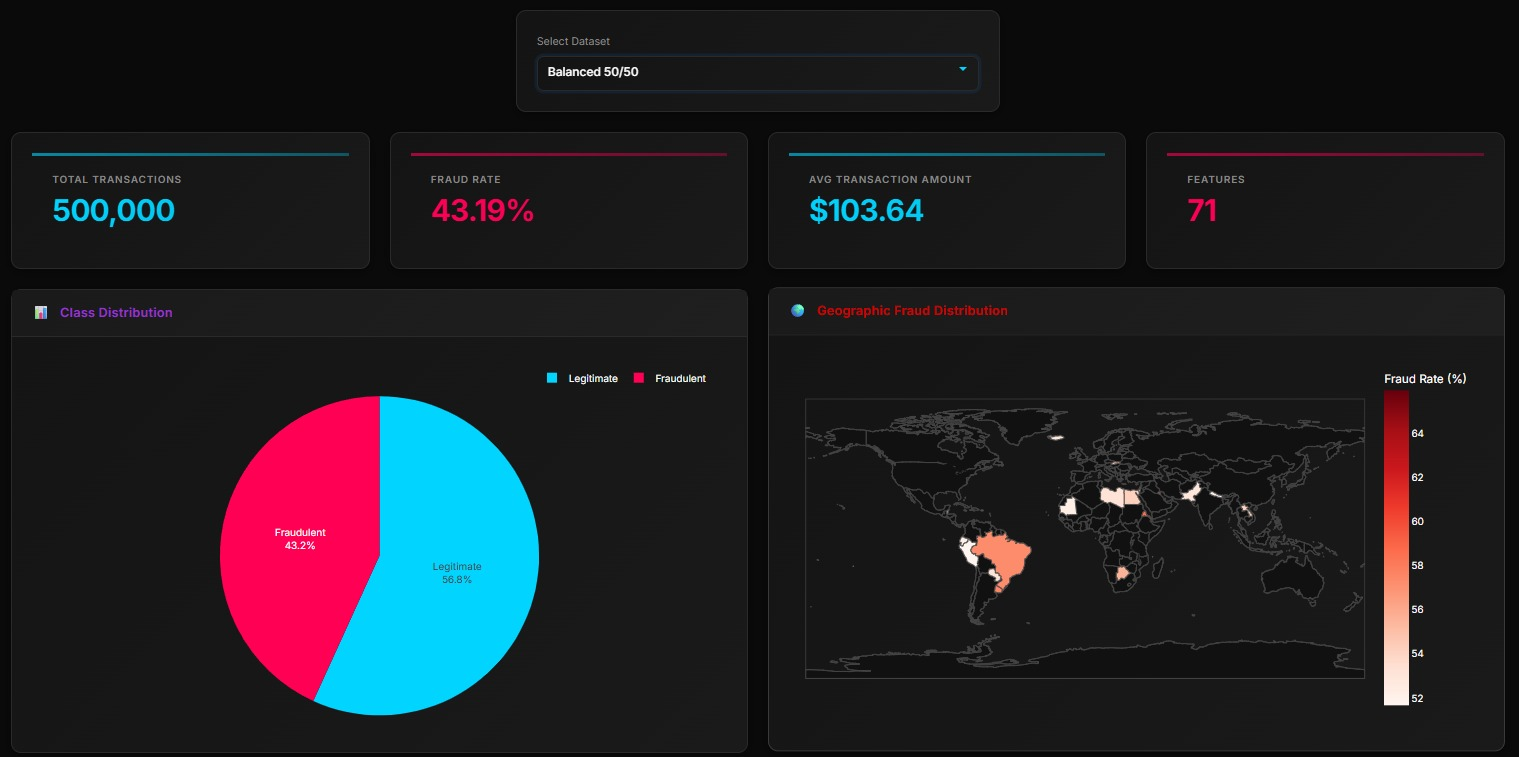
\includegraphics[width=1\linewidth]{imagenes/dashboard_eda.jpeg}
    
\end{figure}
\subsection{Objective of the EDA page}

This page focuses on \textbf{understanding patterns behind fraud}. The goal is not to classify, but to compare the fraudulent and the legitimate behavior, highlighting variables and contexts that are useful for model design. It is an expansion of the first page, Overview.

The section is fully interactive and allows the client to switch between different processed data (balanced vs realistic proportions) to understand how preprocessing decisions affect the fraud patterns.

\subsection{User Control: Dataset Selection}

A dropdown menu allows selecting between multiple datasets: 
\begin{itemize}
    \item balanced 50/50
    \item balanced 66/33
    \item random oversampling
    \item original class proportion
\end{itemize}

These training datasets were balanced by us, generating synthetic data, to evaluate their impact on model performance. Including them in the EDA allows users to explore how different data affects transaction distributions.

\subsection{Main Elements of the EDA Page}

\textbf{KPI Summary}
Four KPI cards summarize the selected dataset:

\begin{itemize}
    \item Total Transactions: number of rows in the selected dataset.
    \item Fraud Rate: average of the \texttt{Class} variable , display as a percentage (the fraudulent transactions over the total transactions).
    \item Average Transaction Amount.
    \item Features: number of usable modeling variables, excluding IDs and metadata columns.
\end{itemize}

\textbf{Class Distribution}
A pie chart shows the proportion of \texttt{Class=0} (legitimate) vs. \texttt{Class=1} (fraud). It is a reminder of the class imbalance challenge and helps comparing dataset versions quickly.

\textbf{Geographic Fraud Distribution}
Using a world map to show the fraud rates, according to the smooth fraud rate percentage, per country using a color scale. The hover shows: 
\begin{itemize}
    \item Fraud Rate (\%)
    \item Total Transactions
    \item Fraud Count
\end{itemize}

\textbf{Transaction Amount distribution}
This chart replicates the histogram shows in the Overview page, applied to the selected dataset. A logarithmic scale is used, due to the skewness of amount, to compare the distributions of legitimate and fraudulent transactions.

\textbf{Time of Day Analysis (fraud rate by hour)}
This graph also replicates the temporal plot in the Overview. They compute the fraud rate by extracting the hour from \texttt{timestamp} and then grouping by hour:
\[
\text{fraud\_rate}(h) = 100 \cdot \mathbb{E}[\texttt{Class} \mid \text{hour}=h]
\]
The chart shows when fraud is relatively more frequent (at dawn), which is useful for time-based strategies.

\textbf{PCA Feature Relationships (correlation analysis)}
Two plots present the anonymized PCA features V1-V28:

\begin{itemize}
    \item Correlation matrix (heatmap): shows how PCA components relate to each other, to identify patterns and dependencies in the data.
    \item Correlation with Class (bar chart): computes the correlation between each PCA feature and \texttt{Class}, then sorts by absolute correlation to highlight which PCA dimensions are most related with fraud.
\end{itemize}

This does not imply causality, but it helps highlight features with stronger linear relationships. PCA variables should be independent, however, since the original data generation is unkown, this analysis is included to check for unexpected relationships or potential leakage.

\section{Modeling and Performance}
\begin{figure}
    \centering
    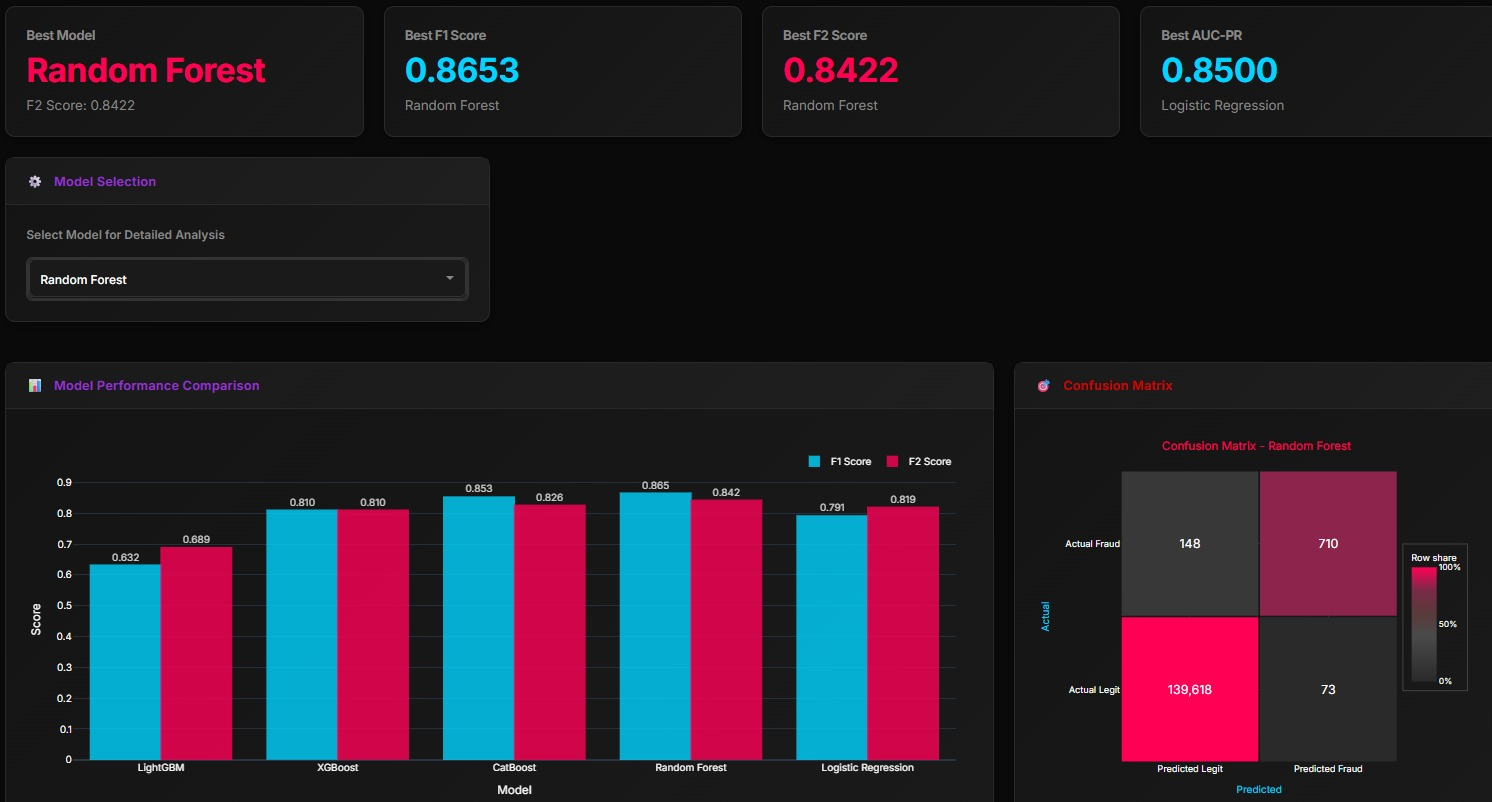
\includegraphics[width=1\linewidth]{imagenes/dashboard_modeling.jpeg}
\end{figure}

\subsection{Objective of the Modeling Page}

This page shifts the focus from data understanding to model evaluation. While the Overview page describes the general data, the EDA explores underlying patterns of each dataset, this page answers a key question for stakeholders: 

\begin{quote}
\emph{Which fraud detection model performs best under realistic conditions, and what trade-offs does it imply?}
\end{quote}
All the results shown on this section are based on the models we have defined, and explained in the Modeling part. The dashboard does not perform training or tuning, both lengthy processes; it only presents and compares the final model performance.

Our primary objective is to maximize fraud detection capacity, prioritizing the identification of fraudulent transactions while keeping operational impact under control.

\subsection{Dataset Context}
The dataset selected for the evaluation of all the models presented on this page is the \textbf{Same Proportion dataset} because it preserves the original class distribution of the transaction data. It reflects the highly imbalanced nature of real world scenarios.

This choice ensures realistic metrics, not inflated by artificial balanced techniques. As a result, performance values should be interpreted as conservative but viable. 

\subsection{Main Elements of the Modeling Page}

\textbf{Model Performance KPIs}
To follow the style of our entire dashboard, four KPI cards summarize the best performing models according to different metrics:

\begin{itemize}
    \item Best Model: model selected as the overall reference.
    \item Best F1 Score: model achieving the best balance between precision and recall.
    \item Best F2 Score: model optimized for recall, prioritizing fraud detection.
    \item Best AUC-PR: model with the highest area under the Precision--Recall curve, robust to class imbalance.
\end{itemize}

\textbf{Model Selection Control}
A dropdown menu allows clients to interact and choose the model they want to inspect with more detailed. Once it is selected, the confusion matrix and ROC and PR curves are updated, supporting comparison of trade-offs among models.

\textbf{Performance comparison chart}
A grouped bar chart compared F1 and F2 scores across all trained models, making it easier to identify models that maximize recall versus models that are more conservative (higher F1). This can be critical in our scenario, as a false negative fraud is usually more costly.

\textbf{Confusion matrix}
This matrix shows how classification match the ground truth. It is row-normalized so each row sums to 100\% .
It is a clear way of comparing the False Negatives (missed fraudulent transactions) and the False Positives (legitimate transactions flagged as fraud).

\textbf{ROC Curve}
Summarizing the relationship between True Positive Rate and False Positive Rate across thresholds and reports the ROC-AUC score. 

\textbf{Precision - Recall Curve}
It provides the most informative view under severe imbalance, focusing on the fraud class. It shows how precision decreases as recall increases when the decision threshold is reduced.

\textbf{Detailed Metrics Table}
A final table consolidates all key metrics per model, highlighting the best values:
\begin{figure}
    \centering
    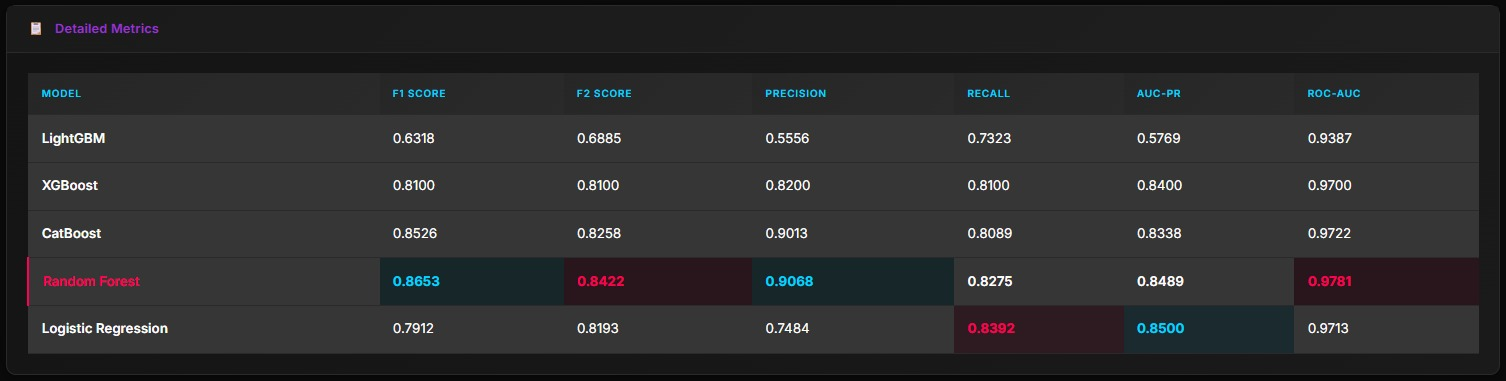
\includegraphics[width=1\linewidth]{imagenes/dashboard_modeling2.jpeg}
\end{figure}

\section{Fraud Simulator}
\subsection{Objective of the Fraud Simulator Page}

The Fraud Simulator page is conceived as a \textbf{demonstration layer} that connects the modeling results with a potential real-world usage scenario. Its objective is not to provide a production-ready tool, but to illustrate how the selected fraud detection model could be applied to individual transactions in an interactive way for the user.

This page aims to help non-technical stakeholders understand how model predictions translate into operational decisions, using a simplified and controlled setting.

\subsection{Main Elements of the Fraud Simulator Page}

\textbf{Transaction Input Panel}  
The simulator includes a form where the user can manually define a transaction scenario. The current inputs are intentionally limited to keep the interaction simple:
\begin{itemize}
    \item Transaction amount.
    \item Customer country.
    \item Time of day (hour).
\end{itemize}
These inputs are representative of common risk drivers and allow users to explore how changes in transaction context affect the model output.

\textbf{Model Inference Logic}  
The simulator relies on the final selected model (Random Forest trained on the Same Proportion dataset). An attempt was made to transform user inputs into a feature vector compatible with the model, using neutral or representative values for non-specified variables. This step would mimic the feature preparation process that would occur in a real-time scoring pipeline. However, since the final model relied on many anonymized PCA variables, it was difficult to establish a link to the user inputs. Due to this, another simpler model was trained for demonstration purposes solely based on the inputs.

\textbf{Prediction output and confidence}  
For each simulated transaction, the page displays a binary decision to either approve the transaction or block it due to detected fraud, in which case it also calculates the associated fraud probability. This output is designed to be easily interpretable, avoiding technical metrics and focusing on actionable results.

\textbf{Operational recommendation}  
Alongside the prediction, a short recommendation is shown (e.g., approve the transaction or block and review). This reinforces the idea that model outputs are inputs to decision-making processes, not decisions by themselves.

\textbf{Model transparency panel}  
Basic information about the model used (model type and number of features) is displayed to provide context and transparency during the demo, without exposing implementation details.

\chapter{DEVELOPMENT OF STRATEGIES AND RISK MANAGEMENT MODEL}

\section{Strategic context: The transaction from the block to the identity management}

In today's financial ecosystem, fraud detection has evolved from a purely defensive cost center into a critical revenue enabler. The implementation of the predictive model developed in this project, based on \textit{ensemble algorithms} (XGBoost, CatBoost, Random Forest...), addresses an imperative business need: the mitigation of Operational Risk without compromising User Experience (UX)

The traditional paradigm based on static rules (\textquotedblleft If Amount > \$X, Block\textquotedblright) has become obsolete. According to the \textit{'True Cost of Fraud Study'} by LexisNexis Risk Solutions (2023), the real cost of fraud for financial institutions is not equivalent to the nominal value of the loss. The cost multiplier stands at \$4.41 USD for every \$1 USD defrauded \cite{Lexisnexis2023a}. This multiplier is composed of:



\begin{itemize}
    \item Fund restitution costs.
    \item Administrative investigation expenses (OpEx).
    \item Legal and regulatory compliance costs.
    \item Loss of trust and brand reputation.
\end{itemize}


Consequently, the strategy proposed in this document does not simply seek to \textquotedblleft stop transactions\textquotedblright, but rather to optimize capital allocation through \textbf{Risk-Based Authentication (RBA)}. By utilizing the key predictor variables identified in our model (V14, customer country, and amount), we propose a dynamic system that discriminates between actual fraud and legitimate anomalies with a precision superior to the current system.


\section{Design of Prevention Strategies and Regulatory Compliance (PSD2)}

The cornerstone of this proposal is the alignment of the mathematical model with the European Union's \textit{Payment Services Directive 2 (PSD2)}, specifically with the \textit{Regulatory Technical Standards (RTS)} on Strong Customer Authentication (SCA).

The model will act as the decision engine for applying the \textit{Transaction Risk Analysis (TRA) exemption}, as stipulated in Article 18 of the \textit{European Banking Authority (EBA)} delegated regulation.



\subsection{Operational Flow Segmentation (Traffic Light Approach)}

Based on the probability score (\(P_f\)) generated by the Random Forest model, we will segment transactional traffic into three action \textit{clusters}, designed to maximize conversion rates and minimize friction:

\subsubsection{\textquotedblleft Frictionless\textquotedblright Flow (Direct Approval Zone)}

\textbf{Model Criterion:} Transactions with \(P_f < 0.50\) (Conservative threshold adjusted for a low False Positive Rate).  

\textbf{Business Action:} Invisible approval. No 2FA (Two-Factor Authentication) requested.  

\textbf{Regulatory Justification:} The predictive model allows the entity’s overall fraud rate to remain below the 6 to 13 basis points (bps) required by the EBA to exempt transactions of up to €100 and €250, respectively, from SCA \cite{eba2023}.
 

\textbf{Financial Impact:} Estimated 5-10\% increase in the approval rate for genuine customers. According to Visa data, merchants that maximize the use of frictionless programs observe an immediate reduction in shopping cart abandonment \cite{visa2023a}.

\subsubsection{\textquotedblleft Smart Challenge\textquotedblright Flow (Strong Authentication Zone)}

\textbf{Model Criterion:} Transactions with \(0.50 \le P_f < 0.85\).  

\textbf{Business Action:} Activation of the 3-D Secure 2.0 protocol. The customer is prompted for a proof of life (biometrics) or an OTP code.  

\textbf{Rationale:} This segment contains legitimate but atypical transactions (e.g., travel or high-value purchases). Blocking them directly would generate a high \textit{Customer Insult Rate}.

\textbf{Market Support:} A study conducted by Javelin Strategy \& Research reveals that 33\% of customers permanently abandon a financial institution after a false decline \cite{javelin2023a}. The \textquotedblleft Challenge\textquotedblright instead of \textquotedblleft Denial\textquotedblright strategy preserves \textit{Customer Lifetime Value (CLV)}.

\subsubsection{Containment Flow (Blocking/Investigation Zone)}

\textbf{Model Criterion:} Transactions with \(P_f \ge 0.85\).  

\textbf{Business Action:} Automatic rejection (for scores \(> 0.95\)) or submission to the analyst queue (0.85--0.95).  

\textbf{Model Finding:} Our \textit{Feature Importance} analysis demonstrates that when variables V14 and amount present extreme negative values, the probability of fraud is near certainty. This allows for automated rejection without human intervention, reducing the operational burden.

\section{Process Re-engineering: OpEx Optimization and Operational Efficiency}

The implementation of the model is not merely a technological upgrade, but a restructuring of the risk department's operational efficiency.




\subsection{Alert Fatigue Reduction}

Currently, linear rule-based systems generate an unmanageable volume of alerts. In the industry, a 15:1 ratio (15 manual reviews to find 1 actual case of fraud) is common. This oversaturates analysis teams, leading to \textit{alert fatigue} and human error.

The proposed model, by integrating decision tree algorithms, captures non-linear relationships between variables that simple rules overlook.

\textbf{Projected Impact:} An estimated 60\% reduction in manual alert volume, concentrating human capital solely on cases within \textquotedblleft Segment C\textquotedblright{} (high probability).  

\textbf{Economic Benefit:} Reduction in the \textit{Cost per Investigation (CPI)}. Assuming an industry-standard cost of \$10 USD per manual review, the reduction in unnecessary alerts directly impacts the \textit{Operating Expenses (OpEx)} line of the income statement.

\subsection{Continuous Learning Cycle (Human-in-the-Loop)}

A feedback protocol will be established where the analysts' final decisions on doubtful cases (\textquotedblleft Yellow Zone\textquotedblright) will be fed back into the training dataset.

\textbf{Objective:} To mitigate the risk of \textit{Concept Drift} (model degradation). Since fraud patterns evolve rapidly, this cycle ensures that the model learns new attack typologies (e.g., synthetic fraud) detected by humans, updating the weights of critical variables such as V14.


\section{Model Governance and Explainability (XAI)}

To ensure the viability of the deployment in a regulated environment, the strategy includes an \textit{Explainable Artificial Intelligence (XAI)} framework, aligned with the \textit{NIST AI Risk Management Framework} \cite{nist2023} and the \textit{EU AI Act}.



\subsection{Decision Transparency (SHAP Values)}

Unlike traditional \textquotedblleft black boxes\textquotedblright{}, our implementation utilizes SHAP (\textit{SHapley Additive exPlanations}) values to break down each rejection decision.

\textbf{Practical Application:} When the model denies a transaction, it does not only return a score of 0.99, but also provides a precise justification:  

\begin{quote}
\textit{\textquotedblleft Denied because variable V14 (correlated with geolocation/behavior) deviates 3 standard deviations from the user's mean.\textquotedblright}
\end{quote}

\textbf{Business Value:} This allows customer service agents to explain the reason for the block to the end user (where regulation permits) and facilitates internal \textit{Fairness Audits}, ensuring the model does not discriminate based on protected variables.




\section{Estimated Impact Analysis and ROI Projections}

To validate the investment in this analytical infrastructure, we present a \textit{Return on Investment (ROI)} estimate based on simulated scenarios using the model's validation data.

\subsection{Financial Impact Matrix}

    \begin{table}[h!]
        \centering
        \small 
        \renewcommand{\arraystretch}{1.3} 
        
        \begin{tabularx}{\textwidth}{@{} l c c >{\raggedright\arraybackslash}X @{}}
            \toprule
            \textbf{Key Performance Indicator (KPI)} & 
            \textbf{\shortstack{Baseline Scenario\\(Rules)}} & 
            \textbf{\shortstack{ML Scenario\\(XGBoost)}} & 
            \textbf{Economic Impact} \\
            \midrule
            
            Detection Rate (Recall) & 
            $\sim$60\% & 
            $\sim$77.27\% (Projected) & 
            Direct reduction in losses from undetected fraud (Write-offs). \\
            \addlinespace
            
            False Positive Rate (FPR) & 
            $\sim$5.0\% & 
            $\sim$0.03\% & 
            Revenue preservation from approved legitimate transactions. \\
            \addlinespace
            
            Analyst Efficiency & 
            10 alerts/hour & 
            25 alerts/hour & 
            Higher fraud density in reviewed alerts. \\
            \bottomrule
        \end{tabularx}
        \caption{KPI Performance Comparison}
    \end{table}
    




\subsection{Savings Quantification (Cost Model)}

Using the \textit{Oxford Economics} framework on losses from false declines, we estimate that the financial savings stem from two primary sources:

\begin{enumerate}
    \item \textbf{Defensive Savings (Hard Savings):}  
    By increasing \textit{Recall} from 60\% to 77\%, an additional 17\% of fraud volume is intercepted. Applying the LexisNexis multiplier (4.41x), every \$100,000 USD of additional fraud stopped translates into \$441,000 USD in net savings for the institution.

    \item \textbf{Offensive Savings (Revenue Protection):}  
    Reducing \textit{False Positives} from 5\% to 0.03\% implies \textquotedblleft rescuing\textquotedblright{} 4.97\% of the transactional customer base that was previously erroneously blocked.

    \textbf{Impact Calculation:}  
    \[
    \text{Savings} = (\text{Total Transactional Volume}) \times 4.97\% \times (\text{Average Ticket})
    \]
    This cash flow represents pure operating profit that was previously lost to the competition (\textit{Wallet Share Loss}).
\end{enumerate}







\subsection{Deployment Recommendation (Roadmap)}

A phased deployment via a \textit{Champion/Challenger (A/B Testing)} strategy is recommended to minimize operational risk and integrate the model in a controlled manner:

\begin{itemize}
    \item \textbf{Phase 1 (Weeks 1--4):} The model runs in \textit{Shadow Mode}, scoring transactions in real-time without taking actions, with the objective of validating the stability of the V14 and customer country variables.
    
    \item \textbf{Phase 2 (Weeks 5--8):} The model assumes decision-making for 10\% of the traffic, specifically within the low-risk segment.
    
    \item \textbf{Phase 3 (Go-Live):} Full migration of the decision engine, maintaining the legacy rules solely as a \textquotedblleft Safety Net\textquotedblright{} for outlier cases not represented in the training dataset.
\end{itemize}








\chapter{Economic Viability Analysis and Return on Investment (ROI)}

\section{Methodological Framework: From the Confusion Matrix to the Cost Matrix}

The evaluation of a \textit{Machine Learning} model's success in the financial sector cannot be limited to traditional statistical metrics such as \textit{Accuracy} or \textit{AUC-ROC}. To determine the feasibility of the production deployment for RandomForest algorithms, we have adopted a \textbf{Weighted Cost Matrix} approach, where prediction errors are penalized based on their real impact on the entity's income statement.

Unlike a sterilized academic environment, errors in transactional banking are asymmetric:

\begin{itemize}
    \item \textbf{Cost of a False Negative} (\(C_{FN}\)): Undetected fraud. This entails direct loss of capital, administrative costs, and regulatory fines.
    \item \textbf{Cost of a False Positive} (\(C_{FP}\)): Legitimate customer blocked. This entails opportunity cost, operational friction, and the deterioration of the customer's \textit{Lifetime Value (LTV)}.
\end{itemize}

The financial optimization function (\(J\)) guiding our strategy does not seek to minimize overall error, but rather the \textbf{Expected Total Cost} (\(E[C]\)):

\[
J = \min \left( N_{FN} \cdot C_{FN} + N_{FP} \cdot C_{FP} + C_{Tech} \right)
\]

Where \(C_{Tech}\) represents the computational and maintenance costs of the inference infrastructure.



\section{Unit Economics: The Fraud Cost Multiplier}

To quantify \(C_{FN}\), we rely on the industry standard established by the report \textit{\textquotedblleft True Cost of Fraud Study: Financial Services Edition\textquotedblright} (LexisNexis, 2023) \cite{lexisnexis2023a}. This study reveals that the actual cost to a financial institution for every dollar defrauded is significantly higher than the nominal loss.

\subsection{The 4.41x Multiplier}

The LexisNexis analysis establishes a multiplier of 4.41. This means that for every \$1.00 USD of fraudulent transaction that the current rules-based system misses, the entity incurs a total cost of \$4.41 USD.

The breakdown of this multiplier, as applied to our model, includes:

\begin{enumerate}
    \item \textbf{Principal Loss (1.00):} The transaction amount absorbed by the bank (\textit{liability shift}).
    \item \textbf{Investigation and Recovery Costs (2.10):} Analyst man-hours, case management software, and telecommunication costs to verify identity.
    \item \textbf{Legal and Compliance Costs (0.90):} Reporting to regulators, PSD2/GDPR fine provisions, and audits.
    \item \textbf{Asset Replacement (0.41):} Issuance and shipping of new physical cards and digital credentials.
\end{enumerate}

\textbf{Model Implication:} The high sensitivity (\textit{Recall}) achieved by our Random Forest model, driven by the V14 variable, directly addresses this multiplier, generating exponential and non-linear savings.

\section{The Hidden Cost: \textquotedblleft Insult Rate\textquotedblright{} and Customer Churn}

While fraud is costly, the incorrect blocking of legitimate customers (\(C_{FP}\)) represents the greatest long-term risk to revenue.

\subsection{Quantifying the \textquotedblleft False Decline\textquotedblright}

According to the joint study by \textit{Checkout.com} and \textit{Oxford Economics} (2022), global losses due to false declines amounted to \$50.7 billion, surpassing losses from actual fraud in certain sectors \cite{oxford2022}.

In our financial analysis, we impute a cost to each False Positive based on two factors derived from \textit{Javelin Strategy \& Research} \cite{javelin2023b}:

\begin{itemize}
    \item \textbf{Immediate Transaction Loss:} Lost interchange margin (\textit{Interchange Fee}).
    \item \textbf{Churn and LTV Damage:} It is estimated that 33\% of customers abandon the institution or relegate the card to the \textquotedblleft Back of Wallet\textquotedblright{} after a false decline.
\end{itemize}

The total cost of a False Positive is defined as:

\[
C_{FP} = \text{Margin} + (\text{Average LTV} \times \text{Churn Probability})
\]

By reducing the False Positive Rate from 5\% (static rule baseline) to 0.03\% (proposed model), the institution's future cash flow is directly preserved.



\section{Financial Simulation: Comparative Scenario (P\&L Impact)}

The following presents a monthly \textit{Profit and Loss (P\&L)} projection, assuming a hypothetical transactional volume of 100,000 operations and an average \textit{ticket} of \$100 USD.

\subsection{Financial Results Summary}

\begin{table}[h!]
    \centering
    \footnotesize
    \renewcommand{\arraystretch}{1.4}
    
    \begin{tabularx}{\textwidth}{@{} l c c >{\raggedright\arraybackslash}X @{}}
        \toprule
        \textbf{Financial Concept} & 
        \textbf{\shortstack{Scenario A\\Current (Rules)}} & 
        \textbf{\shortstack{Scenario B\\Proposed ML}} & 
        \textbf{Monthly Delta} \\
        \midrule
        
        Accuracy & 95.00\% & 99.84\% & +4.84 pp \\
        
        Total Fraud Exposure & \$500,000 \scriptsize{(5\% attack rate)} & \$500,000 & -- \\
        
        Intercepted Fraud & \$300,000 \scriptsize{(60\% Recall)} & \$390,000 \scriptsize{(78\% Recall)} & +\$90,000 \\
        
        Net Fraud Loss & \$200,000 & \$110,000 & -- \\
        \addlinespace
        
        \textbf{1. Cost of Fraud (4.41x)} & \$882,000 & \$485,100 & \textbf{\$396,900 Savings} \\
        
        False Positives & 4,750 \scriptsize{(5\% rate)} & 28 \scriptsize{(0.03\% rate)} & -4,722 Customers \\
        
        \textbf{2. Churn Loss (LTV)} & \$156,750 & \$924 & \textbf{\$155,826 Preserved Revenue} \\
        
        \textbf{3. Manual Review (OpEx)} & \$50,000 & \$5,000 & \textbf{\$45,000 OpEx Savings} \\
        
        \midrule
        \textbf{NET IMPACT} & \textbf{\$1,088,750} & \textbf{\$491,024} & \textbf{ROI: +\$597,726/mo} \\
        \bottomrule
    \end{tabularx}
    \caption{Financial Impact Analysis and ROI}
\end{table}

\subsubsection*{Methodological Notes and Justification:}

The figures presented in the table above are derived from the following strategic pillars:

\begin{itemize}
    \item \textbf{Total Fraud Cost (4.41x Multiplier):} Following the \textit{LexisNexis (2023)} study, for every dollar of Net Fraud Loss (money that leaves the entity), a multiplier of 4.41 is applied to account for restitution, legal fees, and administrative burden. By increasing \textit{Recall} to 78\% via RandomForest, we reduce the net loss, yielding a \textbf{Hard Saving} of \$396,900.
    
    \item \textbf{Churn Calculation and Revenue Preservation:} Based on \textit{Javelin Strategy \& Research}, we assume a 33\% abandonment rate for customers experiencing a False Positive. The loss is calculated as: \textit{FPs $\times$ 0.33 $\times$ \$100 (conservative LTV)}. The drastic reduction of the FPR from 5\% to 0.03\% effectively eliminates the leakage of legitimate customers.
    
    \item \textbf{OpEx Efficiency:} Current manual review costs are estimated at \$10 per alert. The machine learning model's precision allows for a 90\% reduction in the volume of alerts sent to the analyst queue, converting a significant operational cost into \textbf{Direct Operating Profit}.
\end{itemize}



\subsection{ROI Interpretation}

The implementation of the model generates a positive cash flow of \$597,726 per month compared to the current situation. This result represents not only \textit{cost savings}, but also \textbf{operational margin protection}.  

The return on the technological investment required to deploy Random Forest (infrastructure, servers, and data engineering costs) would be recouped in less than 10 days of operation—a \textit{Payback Period} of less than one month.

\section{Operational Efficiency and Resource Reallocation (OpEx)}

Beyond direct financial losses, the model positively impacts the operational cost structure (\textit{OpEx}), specifically the \textbf{Cost per Investigation (CPI)}.

\subsection{Human Capital Optimization}

Currently, fraud analysts spend 80\% of their workday reviewing alerts that turn out to be false positives (\textit{Noise}).

\begin{itemize}
    \item \textbf{Current Situation:} An analyst reviews 50 alerts per day, 45 of which are legitimate customers. Their talent is spent on repetitive, low-value-added tasks.
    \item \textbf{Model-Driven Situation:} By filtering out the noise through the high precision of the V14 and customer country variables, analysts receive enriched alerts with a significantly higher probability of fraud.
\end{itemize}

\textbf{Impact:} This transformation allows for a redefinition of the analyst's role from \textquotedblleft Transaction Reviewer\textquotedblright{} to \textquotedblleft Financial Crime Investigator,\textquotedblright{} focusing on more complex schemes such as money laundering or synthetic fraud, thus providing higher strategic value to the bank.

\section{Sensitivity and Stress Analysis}

To ensure the financial robustness of the proposal, \textit{stress tests} were conducted by varying the key assumptions of the economic model:

\begin{itemize}
    \item \textbf{Conservative Scenario (3.0x Multiplier):}  
    Even when reducing the fraud cost multiplier to 3.0x—assuming extreme efficiencies in recovery—the model maintains monthly savings exceeding \$500,000, preserving a positive ROI.
    
    \item \textbf{Massive Attack Scenario (Spike):}  
    In the event of a \textit{botnet} attack that doubles the volume of fraud attempts, the ML-based system scales automatically without requiring the linear hiring of additional analysts, demonstrating operational elasticity substantially superior to manual rule-based systems.
\end{itemize}



\chapter{Model Risk Governance, Robustness, and Regulatory Compliance}

\section{Model Risk Management (MRM) Framework}

The implementation of black-box machine learning algorithms (\textit{Black-box models}) such as XGBoost and Random Forest introduces a new category of operational risk. To mitigate this risk, our deployment strategy adheres to the principles of the Federal Reserve’s \textbf{SR 11-7} guidance (\textit{Supervision and Regulation Letter}) on \textit{Model Risk Management} \cite{fed2011}.

This framework dictates that the model should not be treated as a static asset, but as a \textbf{continuous lifecycle} that requires independent validation and performance monitoring. System robustness depends not only on initial accuracy but on its ability to maintain that accuracy in the face of changes in the economic environment and emerging fraud patterns.

\section{Limitations Analysis: Temporal Bias and Seasonality}

It is imperative to declare a structural limitation in the current training phase: the \textbf{time window} of the data. The model has been calibrated using a narrowly defined transactional set (approximately 48 hours, in accordance with industry-standard datasets).

\subsection{Seasonal Overfitting Risk}

Financial spending patterns exhibit strong weekly and monthly cyclicity (e.g., higher leisure volume on Fridays or utility payments at the end of the month).

\textbf{Risk:} There is a possibility that the model has learned idiosyncratic patterns specific to the training days rather than generalizable fraud relationships. This could result in \textit{Performance Decay} if deployed on days with distinct consumption behavior, such as \textquotedblleft Black Friday.\textquotedblright

\textbf{Mitigation Strategy (Stress Testing):}  
Following the guidelines of the \textit{Basel Committee on Banking Supervision} regarding stress testing, an \textquotedblleft Out-of-Time (OOT)\textquotedblright{} validation is proposed prior to \textit{Go-Live}.

\textbf{Technical Action:} The model will not be approved for production until it is validated against a \textquotedblleft Challenger Dataset\textquotedblright{} covering a full billing cycle (30 days), ensuring that key predictive variables (V14, customer country) maintain their discriminatory power outside the original temporal sample.

\section{Monitoring Drift and Concept Drift}

Fraud is a dynamic adversarial phenomenon. Unlike image recognition (a cat always looks like a cat), fraud patterns actively evolve to evade detection mechanisms.

\subsection{Concept Drift Detection}

To prevent silent model obsolescence, a surveillance system based on the \textbf{Population Stability Index (PSI)} will be implemented:

$$PSI = \sum \left( ( \%Actual - \%Expected ) \times \ln\left( \frac{\%Actual}{\%Expected} \right) \right)$$

\textbf{Action Protocol:}

\begin{itemize}
    \item $PSI < 0.10$: The model is stable. No action required.
    \item $0.10 \le PSI < 0.25$: Early warning. Variable-level analysis is initiated (V14 is historically the most volatile).
    \item $PSI \ge 0.25$: Critical drift. The \textbf{Emergency Retraining} protocol is activated, and the system temporarily reverts to the rules-based engine (\textit{Fail-safe mode}).
\end{itemize}

This continuous monitoring approach is a key requirement under the \textit{Guidelines on ICT and Security Risk Management} from the \textbf{European Banking Authority (EBA)} \cite{eba2019}.

\subsection{Contingency Protocol (\textit{Circuit Breaker})}

Beyond passive monitoring, an active \textbf{Kill Switch} defense mechanism has been designed. The system will evaluate performance metrics across 24-hour rolling windows and trigger an automatic reversion to the legacy rules engine under two critical conditions:

\begin{itemize}
    \item \textbf{Critical False Positives:} If the False Positive Rate (\textit{FPR}) exceeds the 2\% threshold, threatening massive user experience disruption.
    \item \textbf{Fraud Leakage:} If the Detection Rate (\textit{Recall}) falls below 70\% (validated against reported \textit{chargebacks}).
\end{itemize}

Upon triggering this \textit{Circuit Breaker}, the \textit{Data Ops} team will be immediately notified, and the model will switch to \textit{offline} mode for recalibration, ensuring business continuity without uncontrolled financial risk.


\section{Explainability (XAI) and Ethical Compliance (EU AI Act)}

The opacity of \textit{RandomForest} models presents a regulatory challenge, particularly regarding Article 22 of the \textit{General Data Protection Regulation (GDPR)}—concerning automated decision-making—and the \textit{European Union Artificial Intelligence Act (EU AI Act)}.

\subsection{From Score to Reason: SHAP Implementation}

To guarantee the customer's \textbf{Right to an Explanation}, the \textit{SHAP (SHapley Additive exPlanations)} library has been integrated into the inference pipeline.

\textbf{Mechanism:}  
Whenever the model issues a fraud probability higher than 0.85, the system calculates the marginal contribution of each variable to that specific decision.

\textbf{Use Case:}

\begin{itemize}
    \item \textbf{Input:} Transaction denied.
    \item \textbf{Black Box:} Score = 0.98.
    \item \textbf{XAI Layer:} \textquotedblleft The denial is primarily due to V14 (unusual behavior compared to historical patterns) and V4 (atypical amount for this merchant).\textquotedblright
\end{itemize}

\textbf{Compliance:}  
This mechanism allows compliance officers to audit decisions, demonstrating the absence of bias against protected groups. Furthermore, it ensures alignment with the \textbf{NIST} \textit{AI Risk Management Framework (AI RMF 1.0)} \cite{nist2023b}.

\section{Deployment Strategy: Champion/Challenger Architecture}

To mitigate risks during the transition from the current system to the new model, a \textquotedblleft Big Bang\textquotedblright{} (immediate replacement) approach is discarded. Instead, the \textit{Champion/Challenger} methodology—an industry standard in payment and credit card processing—is adopted.

\begin{enumerate}
    \item \textbf{Phase 1: Shadow Mode.} The model operates in parallel with the current system without affecting live decisions, allowing for the comparison of key metrics (\textit{PSI, Recall, FPR}).
    \item \textbf{Phase 2: Progressive Validation.} Decision-making is enabled for a low-risk subset of traffic.
    \item \textbf{Phase 3: Controlled Go-Live.} Full implementation is achieved, while maintaining traditional rules as a safety net.
\end{enumerate}

\subsection{Technological Integration Architecture}

To ensure the real-time operability required by electronic payment processing, the model will be deployed using a \textbf{containerized microservices architecture}.

\begin{itemize}
    \item \textbf{Low-Latency REST API:} The trained Random Forest model will be serialized and exposed through a REST API (utilizing FastAPI or Flask). This service will receive the transaction feature vector (JSON containing PCA variables, customer country, and amount) and return the fraud score (\(P_f\)) and the SHAP reason code.
    
    \item \textbf{Performance SLA:} Preliminary load tests indicate an inference latency of less than 200ms (\textit{p99}), comfortably meeting the timeouts of standard payment gateways.
    
    \item \textbf{Shadow Mode Implementation:} During the initial phase, this API will consume events from the message bus (Kafka/RabbitMQ) asynchronously, without blocking the primary authorization flow, to validate technical stability.
\end{itemize}


\section{Conclusions and Final Recommendation}

The comprehensive analysis confirms that implementing the \textbf{Random Forest}-based model is not only technically feasible but also financially necessary.

\begin{itemize}
    \item \textbf{Economic Viability:} A positive monthly ROI of \$597,726 is projected, driven by the fraud reduction multiplier (4.41x) and revenue preservation through a lower false positive rate.
    \item \textbf{Strategic Alignment:} The solution ensures PSD2 compliance and enables competitive \textit{Frictionless} user experiences.
    \item \textbf{Risk Control:} Despite training limitations, the governance framework (PSI Monitoring, XAI with SHAP, and phased deployment) keeps risks within the institutional appetite.
\end{itemize}

%\printbibliography


\end{document}
